% ============================================================================
% MASGym: A Co-Evolving Red/Blue Security Gym for Multi-Agent LLM Systems.
% Elsevier (elsarticle) manuscript. See idea_fidelity_report.md and
% topic_signature.json for the LOCKED specification this manuscript must remain
% consistent with (source of truth: idea.pdf).
%
% BUILD: latexmk -pdf main.tex   (or: pdflatex; bibtex; pdflatex; pdflatex)
% NOTE:  elsarticle.cls in this directory is a LOCAL COMPATIBILITY SHIM used
%        because the official class was unavailable offline. For submission,
%        install the official elsarticle.cls and delete the local shim; main.tex
%        compiles unchanged. See TODO_before_submission.md.
% ============================================================================
\documentclass[preprint,12pt]{elsarticle}

% ---- encoding / fonts ----
\usepackage[utf8]{inputenc}
\usepackage[T1]{fontenc}
\usepackage{lmodern}
\usepackage{microtype}

% ---- math ----
\usepackage{amsmath,amssymb,amsthm,mathtools,bm}
\usepackage{xspace}

% ---- lists / tables / floats ----
\usepackage{enumitem}
\usepackage{booktabs,multirow,array}
\usepackage{xcolor}
\usepackage{graphicx}
\usepackage{subcaption}
\usepackage{float}

% ---- graphics: TikZ / PGFPlots ----
\usepackage{tikz}
\usetikzlibrary{arrows.meta,positioning,calc,fit,backgrounds,shapes.geometric,%
  shapes.symbols,decorations.pathreplacing,patterns,matrix,shadows.blur}
\usepackage{pgfplots}
\pgfplotsset{compat=1.18}
\usepgfplotslibrary{groupplots,fillbetween}

% ---- hyperlinks + clever references (order matters: hyperref then cleveref) ----
\usepackage[colorlinks=true,linkcolor=blue!55!black,citecolor=blue!55!black,%
  urlcolor=blue!55!black]{hyperref}
\usepackage{cleveref}

% ---- shared TikZ styles (visual grammar) ----
% ============================================================================
% figures/tikz_styles.tex
% Shared visual grammar for all MASGym figures.
% Colour code (also encoded by shape/pattern for grayscale readability):
%   blue   = honest / normal system component (agents, orchestrator, memory)
%   orange/red = adversarial (colluders, compromised orchestrator, malicious tool, Sybil)
%   green  = defense / blue-team / deterministic checker (trusted evaluation)
%   purple = theory / mathematics
%   gray   = infrastructure / environment harness / background
% Arrow lanes: dataflow (blue), ctrlflow (gray dashed), advflow (red dashed),
%   defflow (green), theoryflow (purple).
% ============================================================================

% ---- palette ----
\definecolor{honest}{RGB}{31,97,164}      % blue
\definecolor{honestbg}{RGB}{219,232,246}
\definecolor{advers}{RGB}{200,63,42}      % red-orange
\definecolor{adversbg}{RGB}{250,224,216}
\definecolor{defense}{RGB}{34,139,80}     % green
\definecolor{defensebg}{RGB}{219,241,226}
\definecolor{theorycol}{RGB}{120,66,161}  % purple
\definecolor{theorybg}{RGB}{233,223,244}
\definecolor{infra}{RGB}{90,90,95}        % gray
\definecolor{infrabg}{RGB}{233,233,236}
\definecolor{amber}{RGB}{214,158,46}
\definecolor{amberbg}{RGB}{250,240,214}

% ---- generic node styles ----
\tikzset{
  >={Latex[length=2.4mm,width=1.8mm]},
  font=\small,
  block/.style={
    rounded corners=2pt, draw=infra!80, fill=infrabg, line width=0.7pt,
    align=center, inner sep=4pt, minimum height=8mm, text width=24mm},
  honestblock/.style={block, draw=honest!85, fill=honestbg, text=black},
  advblock/.style={block, draw=advers!85, fill=adversbg, text=black,
    dash pattern=on 3pt off 1.5pt},
  defblock/.style={block, draw=defense!80, fill=defensebg, text=black},
  theoryblock/.style={block, draw=theorycol!80, fill=theorybg, text=black},
  infrablock/.style={block, draw=infra!80, fill=infrabg},
  amberblock/.style={block, draw=amber!85, fill=amberbg, text=black},
  smalllabel/.style={font=\footnotesize, inner sep=1pt},
  arlbl/.style={midway, fill=white, inner sep=1.5pt, font=\scriptsize},
  % arrow "lanes"
  dataflow/.style={-{Latex[length=2.2mm]}, honest!85, line width=0.9pt},
  ctrlflow/.style={-{Latex[length=2.2mm]}, infra!85, line width=0.8pt,
    densely dashed},
  advflow/.style={-{Latex[length=2.2mm]}, advers!85, line width=1.0pt,
    dash pattern=on 3pt off 1.6pt},
  defflow/.style={-{Latex[length=2.2mm]}, defense!80, line width=1.0pt},
  theoryflow/.style={-{Latex[length=2.2mm]}, theorycol!80, line width=0.9pt},
  grp/.style={rounded corners=4pt, draw=#1!55, line width=0.8pt,
    fill=#1!5, inner sep=6pt},
  grp/.default=infra,
}

% ============================================================================
% Pure-TikZ icons (no external images, no fontawesome dependency).
% Each is a "pic" scaled to ~6mm; call with:  \pic at (x,y) {agenticon};
% ============================================================================

% -- worker agent (rounded robot head) --
\tikzset{
  agenticon/.pic={
    \draw[honest!85, fill=honestbg, line width=0.7pt, rounded corners=1pt]
      (-2.6mm,-2.2mm) rectangle (2.6mm,2.4mm);
    \draw[honest!85, fill=white, line width=0.5pt] (-1.2mm,0.3mm) circle (0.7mm);
    \draw[honest!85, fill=white, line width=0.5pt] (1.2mm,0.3mm) circle (0.7mm);
    \draw[honest!85, line width=0.6pt] (-1mm,-1.3mm) -- (1mm,-1.3mm);
    \draw[honest!85, line width=0.6pt] (0,2.4mm) -- (0,3.4mm);
    \fill[honest!85] (0,3.5mm) circle (0.5mm);
  }
}

% -- orchestrator (hub with crown) --
\tikzset{
  orchicon/.pic={
    \draw[honest!90, fill=honestbg, line width=0.8pt] (0,0) circle (2.7mm);
    \draw[honest!90, fill=honest!25, line width=0.6pt]
      (-2mm,0.6mm)--(-1mm,2.2mm)--(0,0.9mm)--(1mm,2.2mm)--(2mm,0.6mm)--(2mm,-0.4mm)--(-2mm,-0.4mm)--cycle;
    \fill[honest!90] (-2mm,0.6mm) circle (0.35mm);
    \fill[honest!90] (0,0.9mm) circle (0.35mm);
    \fill[honest!90] (2mm,0.6mm) circle (0.35mm);
  }
}

% -- compromised orchestrator (hub with crown + cross) --
\tikzset{
  orchbadicon/.pic={
    \draw[advers!90, fill=adversbg, line width=0.8pt] (0,0) circle (2.7mm);
    \draw[advers!90, fill=advers!20, line width=0.6pt]
      (-2mm,0.6mm)--(-1mm,2.2mm)--(0,0.9mm)--(1mm,2.2mm)--(2mm,0.6mm)--(2mm,-0.4mm)--(-2mm,-0.4mm)--cycle;
    \draw[advers!95, line width=0.9pt] (-1.2mm,-1.0mm)--(1.2mm,-2.4mm);
    \draw[advers!95, line width=0.9pt] (-1.2mm,-2.4mm)--(1.2mm,-1.0mm);
  }
}

% -- Byzantine / attacker node (warning cross) --
\tikzset{
  attackericon/.pic={
    \draw[advers!90, fill=adversbg, line width=0.8pt] (0,0) circle (2.7mm);
    \draw[advers!90, line width=0.9pt] (-1.3mm,-1.3mm)--(1.3mm,1.3mm);
    \draw[advers!90, line width=0.9pt] (-1.3mm,1.3mm)--(1.3mm,-1.3mm);
  }
}

% -- Sybil (two overlapping identity disks) --
\tikzset{
  sybilicon/.pic={
    \draw[advers!85, fill=adversbg, line width=0.7pt] (-1.1mm,0) circle (2.0mm);
    \draw[advers!85, fill=adversbg, line width=0.7pt] (1.1mm,0) circle (2.0mm);
    \draw[advers!85, line width=0.6pt] (-1.1mm,-0.4mm) circle (0.6mm);
    \draw[advers!85, line width=0.6pt] (1.1mm,-0.4mm) circle (0.6mm);
  }
}

% -- shield (defense / blue team) --
\tikzset{
  shieldicon/.pic={
    \draw[defense!85, fill=defensebg, line width=0.8pt]
      (0,3mm) -- (2.4mm,1.6mm) -- (2.4mm,-1mm) -- (0,-3mm)
      -- (-2.4mm,-1mm) -- (-2.4mm,1.6mm) -- cycle;
    \draw[defense!85, line width=0.9pt] (-1.1mm,0.2mm)--(-0.2mm,-1.2mm)--(1.4mm,1.2mm);
  }
}

% -- deterministic checker (clipboard + tick) --
\tikzset{
  checkericon/.pic={
    \draw[defense!85, fill=defensebg, line width=0.7pt, rounded corners=0.6pt]
      (-2mm,-2.7mm) rectangle (2mm,2.7mm);
    \draw[defense!85, fill=white, line width=0.5pt] (-0.9mm,2.3mm) rectangle (0.9mm,3.1mm);
    \draw[defense!85, line width=0.9pt] (-1.2mm,0.2mm)--(-0.3mm,-1.0mm)--(1.4mm,1.4mm);
  }
}

% -- LM tool emulator (cloud with function symbol) --
\tikzset{
  emuicon/.pic={
    \draw[infra!85, fill=infrabg, line width=0.7pt]
      (-2.4mm,-0.6mm) .. controls (-2.8mm,1.4mm) and (-0.9mm,1.9mm) .. (-0.6mm,1.2mm)
      .. controls (0.0mm,2.3mm) and (1.6mm,2.0mm) .. (1.5mm,0.9mm)
      .. controls (2.6mm,0.9mm) and (2.5mm,-0.8mm) .. (1.4mm,-0.9mm)
      -- (-2.0mm,-0.9mm) .. controls (-2.6mm,-0.9mm) and (-2.6mm,-0.6mm) .. (-2.4mm,-0.6mm) -- cycle;
    \node[infra!90, font=\scriptsize\itshape] at (0,0.1mm) {f};
  }
}

% -- tool (gear) --
\tikzset{
  toolicon/.pic={
    \draw[infra!85, fill=infrabg, line width=0.7pt] (0,0) circle (1.9mm);
    \foreach \a in {0,45,...,315}{
      \draw[infra!85, line width=0.8pt] (\a:1.9mm)--(\a:2.8mm);}
    \draw[infra!85, fill=white, line width=0.5pt] (0,0) circle (0.7mm);
  }
}

% -- malicious tool (gear, red, with cross) --
\tikzset{
  toolbadicon/.pic={
    \draw[advers!85, fill=adversbg, line width=0.7pt] (0,0) circle (1.9mm);
    \foreach \a in {0,45,...,315}{
      \draw[advers!85, line width=0.8pt] (\a:1.9mm)--(\a:2.8mm);}
    \draw[advers!90, line width=0.8pt] (-0.9mm,-0.9mm)--(0.9mm,0.9mm);
    \draw[advers!90, line width=0.8pt] (-0.9mm,0.9mm)--(0.9mm,-0.9mm);
  }
}

% -- shared memory store (cylinder/stack) --
\tikzset{
  memicon/.pic={
    \draw[honest!85, fill=honestbg, line width=0.7pt]
      (-2mm,-2.4mm) -- (-2mm,2mm) arc (180:0:2mm and 0.7mm) -- (2mm,-2.4mm)
      arc (0:-180:2mm and 0.7mm);
    \draw[honest!85, line width=0.6pt] (-2mm,2mm) arc (180:360:2mm and 0.7mm);
    \draw[honest!85, line width=0.5pt] (-2mm,0.4mm) arc (180:360:2mm and 0.7mm);
    \draw[honest!85, line width=0.5pt] (-2mm,-1.2mm) arc (180:360:2mm and 0.7mm);
  }
}

% -- poisoned memory (cylinder, red, droplet) --
\tikzset{
  membadicon/.pic={
    \draw[advers!85, fill=adversbg, line width=0.7pt]
      (-2mm,-2.4mm) -- (-2mm,2mm) arc (180:0:2mm and 0.7mm) -- (2mm,-2.4mm)
      arc (0:-180:2mm and 0.7mm);
    \draw[advers!85, line width=0.6pt] (-2mm,2mm) arc (180:360:2mm and 0.7mm);
    \fill[advers!80] (0,-0.2mm) circle (0.55mm);
  }
}

% -- neural net / model --
\tikzset{
  modelicon/.pic={
    \foreach \y in {-1.8mm,0mm,1.8mm}{\fill[honest!80] (-2.2mm,\y) circle (0.5mm);}
    \foreach \y in {-1mm,1mm}{\fill[honest!80] (0,\y) circle (0.5mm);}
    \fill[honest!80] (2.2mm,0) circle (0.5mm);
    \foreach \y in {-1.8mm,0mm,1.8mm}{\foreach \z in {-1mm,1mm}{
      \draw[honest!45, line width=0.3pt] (-2.2mm,\y)--(0,\z);}}
    \foreach \z in {-1mm,1mm}{\draw[honest!45, line width=0.3pt] (0,\z)--(2.2mm,0);}
  }
}

% -- database / dataset --
\tikzset{
  dbicon/.pic={
    \draw[infra!85, fill=infrabg, line width=0.7pt] (-2mm,-2.4mm) rectangle (2mm,2.4mm);
    \draw[infra!85, line width=0.6pt] (-2mm,1.2mm)--(2mm,1.2mm);
    \draw[infra!85, line width=0.6pt] (-2mm,0mm)--(2mm,0mm);
    \draw[infra!85, line width=0.6pt] (-2mm,-1.2mm)--(2mm,-1.2mm);
  }
}

% -- theorem scroll --
\tikzset{
  theoremicon/.pic={
    \draw[theorycol!80, fill=theorybg, line width=0.7pt, rounded corners=1pt]
      (-2mm,-2.6mm) rectangle (2mm,2.6mm);
    \draw[theorycol!80, line width=0.6pt] (-1.2mm,1.4mm)--(1.2mm,1.4mm);
    \draw[theorycol!80, line width=0.6pt] (-1.2mm,0.4mm)--(1.2mm,0.4mm);
    \draw[theorycol!80, line width=0.6pt] (-1.2mm,-0.6mm)--(0.6mm,-0.6mm);
  }
}

% -- human oversight (person) --
\tikzset{
  humanicon/.pic={
    \draw[infra!90, fill=infrabg, line width=0.7pt] (0,1.6mm) circle (1.0mm);
    \draw[infra!90, fill=infrabg, line width=0.7pt]
      (-1.6mm,-2.6mm) .. controls (-1.6mm,0.2mm) and (1.6mm,0.2mm) .. (1.6mm,-2.6mm) -- cycle;
  }
}

% ---- legend helper ----
\newcommand{\legendline}[2]{% #1 style, #2 text
  \draw[#1] (0,0) -- (5mm,0); \node[right, font=\scriptsize] at (5.5mm,0) {#2};}


% ============================================================================
% Theorem environments
% ============================================================================
\theoremstyle{plain}
\newtheorem{theorem}{Theorem}[section]
\newtheorem{lemma}[theorem]{Lemma}
\newtheorem{proposition}[theorem]{Proposition}
\newtheorem{corollary}[theorem]{Corollary}
\theoremstyle{definition}
\newtheorem{definition}[theorem]{Definition}
\newtheorem{assumption}{Assumption}
\theoremstyle{remark}
\newtheorem{remark}[theorem]{Remark}

\crefname{assumption}{Assumption}{Assumptions}
\Crefname{assumption}{Assumption}{Assumptions}

% ============================================================================
% Lightweight algorithm float + pseudocode macros
% (the algorithm/algpseudocode packages were unavailable offline; these macros
%  reproduce a numbered, ruled pseudocode listing and compile everywhere.)
% ============================================================================
\floatstyle{ruled}
\newfloat{algorithm}{tbp}{loa}
\floatname{algorithm}{Algorithm}
\crefname{algorithm}{Algorithm}{Algorithms}
\Crefname{algorithm}{Algorithm}{Algorithms}
\newcounter{algline}
\newlength{\algind}
\newcommand{\algreset}{\setcounter{algline}{0}\setlength{\algind}{0pt}}
\newcommand{\PL}[1]{\par\refstepcounter{algline}\noindent
  \makebox[2.6em][r]{\scriptsize\thealgline:\,}\hspace{0.5em}\hspace{\algind}%
  \ignorespaces#1\strut}
\newcommand{\Ind}{\addtolength{\algind}{1.5em}}
\newcommand{\Ded}{\addtolength{\algind}{-1.5em}}
\newcommand{\kw}[1]{\textbf{#1}}
\newcommand{\comm}[1]{\hfill{\footnotesize\itshape\color{black!55}\(\triangleright\)~#1}}

% ============================================================================
% Notation macros (kept consistent with notation_consistency_check.md)
% ============================================================================
\newcommand{\R}{\mathbb{R}}
\newcommand{\N}{\mathbb{N}}
\newcommand{\E}{\mathbb{E}}
\newcommand{\Prob}{\mathbb{P}}
\newcommand{\indic}{\mathbb{1}}
\newcommand{\Agents}{\mathcal{A}}          % set of agents
\newcommand{\Roles}{\mathcal{R}}           % role set
\newcommand{\Gtop}{\mathcal{G}}            % topology graph
\newcommand{\Vtop}{\mathcal{V}}
\newcommand{\Etop}{\mathcal{E}}
\newcommand{\Nin}{\mathcal{N}^{-}}          % inbound neighbourhood
\newcommand{\Trace}{\tau}                  % global state trace
\newcommand{\TraceSp}{\mathcal{T}}         % trace space
\newcommand{\Statesp}{\mathcal{S}}         % state space
\newcommand{\Predsec}{\Phi}                % system-level security predicate
\newcommand{\Predutil}{\Psi}               % benign-success predicate
\newcommand{\Checker}{\mathsf{C}}          % deterministic checker
\newcommand{\Emu}{\mathcal{E}_{\mathrm{LM}}} % LM tool emulator
\newcommand{\Judge}{\mathsf{J}}            % LLM judge (contrast)
\newcommand{\Advset}{\mathcal{B}}          % adversarial agent set
\newcommand{\betafrac}{\beta}              % adversary fraction
\newcommand{\config}{c}                    % environment configuration
\newcommand{\Configs}{\mathcal{C}}         % configuration space
\newcommand{\ASRs}{\mathrm{ASR}_{\mathrm{sys}}}
\newcommand{\PNAs}{\mathrm{PNA}_{\mathrm{sys}}}
\newcommand{\NRPs}{\mathrm{NRP}_{\mathrm{sys}}}
\newcommand{\CPR}{\mathrm{CPR}}            % compromise-propagation rate
\newcommand{\CSR}{\mathrm{CSR}}            % collusion success rate
\newcommand{\red}{\rho}                    % red policy
\newcommand{\blue}{\delta}                 % blue policy (defense)
\newcommand{\pinf}{p}                      % per-edge propagation probability
\newcommand{\thresh}{\theta}               % threshold (bootstrap percolation)
\newcommand{\kappaem}{\kappa}              % emulation agreement
\newcommand{\defname}{\textsc{MASGym}\xspace}
\newcommand{\corb}{\textsc{CoRB}\xspace}

\journal{Computers \& Security (Elsevier)}

\begin{document}

% ---------------------------------------------------------------------------
% Front matter
% ---------------------------------------------------------------------------
\begin{frontmatter}

\title{\defname: A Co-Evolving Red/Blue Security Gym for Multi-Agent LLM
Systems with Parameterized Collusion, Orchestrator Compromise, and
System-Level Metrics}

\author[rmit]{Thanh Pham\corref{cor1}}
\ead{thanhphamchivn@gmail.com}
\cortext[cor1]{Corresponding author.}
\address[rmit]{School of Computing Technologies, RMIT University, Melbourne, Australia}

\begin{abstract}
Security research on large language model (LLM) agents is bottlenecked by its
instruments: the strongest existing benchmarks---Agent Security Bench (ASB),
AgentDojo, InjecAgent, and the ToolEmu sandbox---are single-agent, and their only
cross-agent vector is a shared memory store. Yet deployed systems are increasingly
orchestrated collectives in which a planner directs workers, agents share memory,
tools are third-party, and coordination is forced. The phenomena that dominate risk
in that regime---collusion among agents, a compromised orchestrator, malicious
tools, Sybil identities, and group-level emergent failure---cannot be produced, let
alone measured, by a single-agent harness. We present \defname, an environment and
evaluation methodology purpose-built for the security of multi-agent LLM systems.
\defname{} contributes: (i) a task suite with heterogeneous roles (orchestrator,
workers, tool-executors, shared-memory store), partial observability, and
\emph{forced-coordination} tasks that no single agent can complete alone, over star,
chain, tree, and mesh topologies at $3$--$50$ agents; (ii) a natively parameterized
adversary model spanning adversary fraction, independent-versus-colluding behaviour,
static-versus-adaptive strategy, orchestrator compromise, malicious tools, Sybils,
and poisoned shared memory; (iii) a system-level metric suite, including a
generalization $\NRPs=\PNAs\cdot(1-\ASRs)$ of ASB's utility--security metric that is
scored against deterministic security predicates over the global state trace, never
an LLM judge on the critical path, so a successful injection cannot hijack the
evaluator; and (iv) \corb, a co-evolving red/blue protocol that alternates attack and
defense proposals and logs their system-level scores. We develop the theory the
instrument requires rather than assuming it: an axiomatic characterization that
singles out the product aggregator and reduces it to ASB's metric at one agent;
an evaluator-integrity theorem separating deterministic checking from LLM-judge
hijack; topology-dependent compromise-propagation bounds and a
collusion-versus-independent separation in the environment's cascade model; a
forced-coordination lower bound; and finite-sample concentration for the estimators.
Built on ToolEmu-style LM emulation (human agreement $\kappaem\approx 0.48$, which we
surface as a first-class caveat) and AgentDojo-style deterministic checks, \defname{}
is an instrument, not a verdict: we never equate a lower system-level attack success
rate with ``secure.'' Because the backbone interface is model-agnostic, we evaluate the
instrument end-to-end on a transparent, clearly-labelled \emph{synthetic} agent emulator
(all headlined output in this version is synthetic and provenance-stamped; a real-backbone
pilot of six open instruct models over twelve configurations is reported separately and
explicitly labelled PILOT). On that emulator the headline claim is measured: defenses effective in
the single-agent regime lose advantage under collusion and compromised-orchestrator
conditions (a per-agent guardrail's relative ASR reduction over no-defense shrinks
$41.6\%\to31.8\%\to27.6\%$ across those contexts; Table~\ref{tab:degradation}); replication
on real backbones and the deferred topologies/scales is the release-phase programme.
\end{abstract}

\begin{highlights}
\item A benchmark environment for \emph{multi-agent} LLM security with heterogeneous
roles, partial observability, and forced-coordination tasks across star, chain, tree,
and mesh topologies at $3$--$50$ agents---phenomena undefined in single-agent harnesses.
\item A natively parameterized adversary: adversary fraction, collusion on/off,
static/adaptive, orchestrator compromised on/off, malicious tools, Sybil identities,
and poisoned shared memory, with system-level compromise objectives.
\item A system-level metric suite generalizing ASB's $\mathrm{NRP}=\mathrm{PNA}\cdot(1-\mathrm{ASR})$
to $\NRPs=\PNAs\cdot(1-\ASRs)$, scored by a deterministic state checker so a
successful injection cannot hijack the evaluator.
\item \corb: a co-evolving red/blue evaluation protocol as a reusable methodology,
logging $(\text{attack},\text{defense})$ trajectories and their system-level scores.
\item Instrument-supporting theory: an axiomatic characterization of the aggregator,
an evaluator-integrity separation, topology-dependent compromise-propagation and
collusion bounds, a forced-coordination lower bound, and estimator concentration---all
under explicitly stated assumptions, with a headline degradation claim measured on a
transparent synthetic emulator and scoped by real-backbone replication.
\end{highlights}

\begin{keyword}
multi-agent LLM security \sep security benchmark and environment \sep co-evolving
red/blue evaluation \sep collusion \sep compromised orchestrator \sep Sybil attack
\sep prompt injection \sep tool emulation \sep deterministic security checking \sep
system-level metrics \sep compromise propagation
\end{keyword}


\end{frontmatter}

% ---------------------------------------------------------------------------
% Body
% ---------------------------------------------------------------------------
\section{Introduction}
\label{sec:intro}

Progress in the security of large language model (LLM) agents has tracked the quality
of the instruments used to measure it. Agent Security Bench (ASB)~\cite{zhang2025asb}
formalized attacks and defenses across an agent's operational stages and introduced a
utility--security metric $\mathrm{NRP}=\mathrm{PNA}\cdot(1-\mathrm{ASR})$;
AgentDojo~\cite{debenedetti2024agentdojo} evaluates an agent under prompt injection
with \emph{deterministic}, state-based \texttt{security()} checks, so that a
successful injection cannot also corrupt the evaluator; InjecAgent~\cite{zhan2024injecagent}
benchmarks indirect prompt injection in tool-integrated agents; and the ToolEmu
sandbox~\cite{ruan2024toolemu} lets a language model emulate arbitrary tool execution
from specifications, trading fidelity for breadth. These instruments are strong, and
they are all single-agent. Their only cross-agent channel is a shared memory store,
and none of them exposes a knob for the phenomena that arise when several agents act
together.

Deployment has moved in the opposite direction. Production systems such as
AutoGen~\cite{wu2023autogen}, MetaGPT~\cite{hong2023metagpt},
CAMEL~\cite{li2023camel}, ChatDev~\cite{qian2024chatdev},
AgentVerse~\cite{chen2024agentverse}, and Magentic-One~\cite{fourney2024magenticone}
are orchestrated \emph{collectives}: a planner directs workers, agents read and write a
shared memory, third-party tools are invoked on the critical path, and many tasks are
structured so that no single agent can finish them alone. In such systems the security
questions that matter are group-level. Do a fraction of agents \emph{collude}? Is the
\emph{orchestrator} itself trusted, or has it been compromised? Can a
\emph{malicious tool}, a \emph{Sybil} identity, or a \emph{poisoned} entry in shared
memory spread through the collective? These are not attributes of any one agent, and
re-running a single-agent benchmark $N$ times does not create them: it produces $N$
independent agents, not a coordinated adversary, an orchestrator with a trust setting,
or a compromise that propagates over a communication topology. The recent
systematization of multi-agent security (MASEC)~\cite{schroederdewitt2025masec} makes
the point sharply---security in multi-agent systems is \emph{non-compositional}, in
that individually safe agents can compose into unsafe systems---and states plainly, in
its Section~4.7, that no multi-agent security benchmark exists, enumerating what one
must provide: heterogeneous roles, partial observability, forced coordination, a
co-evolving red/blue methodology, and group-level emergence metrics. A parallel survey
of multi-agent risks from advanced AI~\cite{hammond2025multiagent} organizes the same
territory into miscoordination, conflict, and collusion, again distinct from
single-agent mitigations. The field therefore cannot currently answer a basic
question: \emph{do single-agent defenses survive multi-agent deployment?}

\paragraph{Contribution.}
We answer the instrument gap directly. \defname{} is, to the best of our knowledge and
within the verified literature, the first environment purpose-built for the security
of multi-agent LLM systems. It is not a new attack and not a new defense; it is an
environment and an evaluation methodology whose scientific object is the controlled
variation of coordination, collusion, and orchestrator variables and the system-level
metrics that quantify their effect. \Cref{fig:architecture} previews the design: a
ToolEmu-style emulation layer supplies breadth of tools; an AgentDojo-style
deterministic checker scores system-level security predicates over the global state
trace, never placing an LLM judge on the critical path; and an orchestration layer
instantiates topology, roles, partial observability, and a parameterized adversary. We
make four concrete contributions and one empirical claim.

\begin{enumerate}[leftmargin=1.5em]
\item \textbf{An environment and task suite for multi-agent LLM security}
(\Cref{sec:system,sec:method}). Heterogeneous roles (orchestrator, workers,
tool-executors, shared-memory store), partial observability, and forced-coordination
tasks, instantiated over star, chain, tree, and mesh topologies at $3$--$50$ agents.
Forced coordination, collusion, compromise propagation, and Sybil pressure are
group-level \emph{by construction} and have no single-agent analogue.

\item \textbf{A natively parameterized adversary model} (\Cref{sec:threat}). A single
configuration vector controls the adversary fraction over agents, independent versus
colluding behaviour, static versus adaptive strategy, orchestrator compromise on/off,
malicious tools, Sybil identities, and poisoned shared memory, with a system-level
compromise objective (unsafe action, exfiltration, or coordination sabotage).

\item \textbf{A system-level metric suite} (\Cref{sec:problem,sec:method}). A
generalization $\NRPs=\PNAs\cdot(1-\ASRs)$ of ASB's metric, together with collusion
success rate, compromise-propagation rate, coordination quality, time-to-detection,
recovery rate, and cost, all measured over the collective rather than per step. Because
$\ASRs$ is scored by a deterministic checker, a successful injection cannot hijack the
evaluator---a property we prove and plan to quantify an LLM-judge ablation against (deferred
to the release phase).

\item \textbf{The \corb{} co-evolving red/blue protocol} (\Cref{sec:algorithm}). A
reusable methodology that alternates a red policy proposing attack configurations from
the parameter space and a blue policy proposing defenses, logging a trajectory of
$(\text{attack},\text{defense})$ pairs and their system-level scores.

\item \textbf{A headline degradation result} (\Cref{sec:experiments}). We measure on a
transparent, clearly-labelled synthetic agent emulator that defenses effective in the
single-agent regime \emph{degrade} under collusion and compromised-orchestrator
conditions: a per-agent guardrail's relative ASR reduction over no-defense shrinks
$41.6\%\to31.8\%\to27.7\%$ across the three contexts (\Cref{tab:degradation}). Real-backbone
replication is the release-phase programme; whether the effect replicates across models and
topologies will confirm or reframe the result.
\end{enumerate}

Because reviewers rightly discount benchmarks whose central metric is asserted rather
than justified, and because the idea's own risk analysis flags construct validity as
the primary threat, we treat the theory as part of the instrument rather than as
decoration. \Cref{sec:theory} states, under explicit assumptions and with honest
proof-status labels, five results: an axiomatic characterization that singles out the
product aggregator among all utility--security combiners and reduces it to ASB's metric
when $N=1$; an evaluator-integrity theorem showing that the deterministic checker's
verdict is invariant to adversarial message content and is therefore not hijackable,
in contrast to an LLM judge; topology-dependent bounds on compromise propagation across
the four topologies together with a strict collusion-versus-independent separation in
the environment's cascade model; a forced-coordination lower bound; and finite-sample
concentration guarantees for the estimators that fix the number of episodes the sweeps
require. None of these results asserts that any real defense is secure or that any
defense provably degrades; they characterize the \emph{measurement}, which is what a
benchmark can honestly own.

\paragraph{Scope and stance.}
\defname{} is an instrument, not a verdict. A lower system-level attack success rate or
a higher system-level NRP is a \emph{measurement under a stated configuration}, not a
certificate of security; we never equate the two. Emulation fidelity is the central
threat to validity---ToolEmu's reported human agreement is $\kappaem\approx 0.48$---and
we surface it as a first-class caveat, route scoring through the deterministic checker,
and report an emulated-versus-real-tools ablation rather than treating emulator verdicts
as ground truth. Following the trusted computing base of the source design, we take the
deterministic state checker and the environment harness to be trusted and give the
emulated tools no real side effects; real-world tool side effects, physical actuation,
and model-weight attacks are out of scope. The remainder of the paper is organized as
follows. \Cref{sec:related} situates \defname{} against single-agent benchmarks,
multi-agent frameworks and attacks, and reinforcement-learning environments;
\Cref{sec:prelim} fixes notation and recalls the ASB, AgentDojo, and ToolEmu
primitives; \Cref{sec:system,sec:threat,sec:problem} give the system model, threat
model, and problem formulation; \Cref{sec:method,sec:algorithm} present the
architecture, metric suite, and \corb{} protocol; \Cref{sec:theory} develops the
theory; \Cref{sec:experiments} specifies the evaluation protocol and the synthetic-model
results; and \Cref{sec:discussion,sec:limitations,sec:ethics,sec:conclusion} discuss
implications, limitations, ethics, and conclusions.

% ============================================================================
% figures/tikz_architecture.tex  --  MASGym system architecture (Fig. 1)
% Three layers: Orchestration (TCB) | Agent collective | Emulation + Checker.
% Lanes: control (gray dashed), data/message (blue), adversarial (red dashed),
% evaluation/trace (green). Icons sit to the LEFT of named nodes.
% ============================================================================
\begin{figure*}[t]
\centering
\resizebox{\textwidth}{!}{%
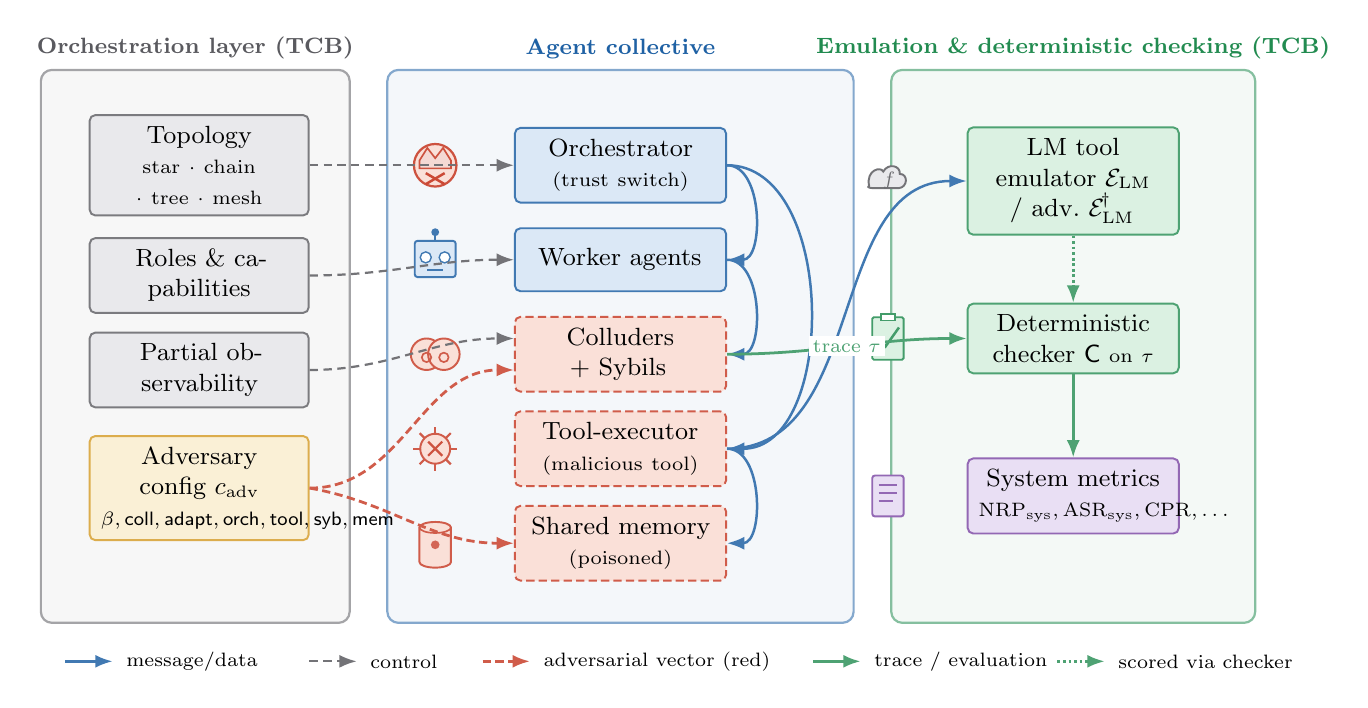
\begin{tikzpicture}[node distance=6mm]

% ---------- Layer group backgrounds (coordinate-based fit) ----------
\begin{scope}[on background layer]
  \node[grp=infra,   fit={(-0.3,-0.1) (3.2,6.5)}, label={[font=\footnotesize\bfseries,infra]above:Orchestration layer (TCB)}] {};
  \node[grp=honest,  fit={(4.1,-0.1) (9.6,6.5)}, label={[font=\footnotesize\bfseries,honest]above:Agent collective}] {};
  \node[grp=defense, fit={(10.5,-0.1) (14.7,6.5)}, label={[font=\footnotesize\bfseries,defense]above:Emulation \& deterministic checking (TCB)}] {};
\end{scope}

% ---------- Column 1: orchestration knobs ----------
\node[infrablock, text width=25mm] (topo)  at (1.5,5.5) {Topology\\ \scriptsize star $\cdot$ chain $\cdot$ tree $\cdot$ mesh};
\node[infrablock, text width=25mm] (roles) at (1.5,4.1) {Roles \& capabilities};
\node[infrablock, text width=25mm] (obs)   at (1.5,2.9) {Partial observability};
\node[amberblock, text width=25mm] (adv)   at (1.5,1.4) {Adversary config $\config_{\mathrm{adv}}$\\ \scriptsize $\betafrac,\mathsf{coll},\mathsf{adapt},\mathsf{orch},\mathsf{tool},\mathsf{syb},\mathsf{mem}$};

% ---------- Column 2: the collective (vertical stack; icons to the left) ----------
\node[honestblock, text width=24mm] (orchp) at (6.85,5.5) {Orchestrator \scriptsize(trust switch)};
\node[honestblock, text width=24mm] (wk)    at (6.85,4.3) {Worker agents};
\node[advblock,    text width=24mm] (col)   at (6.85,3.1) {Colluders + Sybils};
\node[advblock,    text width=24mm] (te)    at (6.85,1.9) {Tool-executor \scriptsize(malicious tool)};
\node[advblock,    text width=24mm] (mem)   at (6.85,0.7) {Shared memory \scriptsize(poisoned)};
\pic at ([xshift=-10mm]orchp.west) {orchbadicon};
\pic at ([xshift=-10mm]wk.west)    {agenticon};
\pic at ([xshift=-10mm]col.west)   {sybilicon};
\pic at ([xshift=-10mm]te.west)    {toolbadicon};
\pic at ([xshift=-10mm]mem.west)   {membadicon};

% message edges within the collective (blue), on the right side
\draw[dataflow] (orchp.east) to[out=0,in=0] (wk.east);
\draw[dataflow] (wk.east)    to[out=0,in=0] (col.east);
\draw[dataflow] (orchp.east) to[out=0,in=0] (te.east);
\draw[dataflow] (te.east)    to[out=0,in=0] (mem.east);

% ---------- Column 3: emulation + checker + metrics ----------
\node[defblock,   text width=24mm] (emubox) at (12.6,5.3) {LM tool emulator $\Emu$ / adv.\ $\Emu^{\!\dagger}$};
\node[defblock,   text width=24mm] (chk)    at (12.6,3.3) {Deterministic checker $\Checker$ \scriptsize on $\Trace$};
\node[theoryblock,text width=24mm] (met)    at (12.6,1.3) {System metrics \scriptsize $\NRPs,\ASRs,\CPR,\dots$};
\pic at ([xshift=-10mm]emubox.west) {emuicon};
\pic at ([xshift=-10mm]chk.west)    {checkericon};
\pic at ([xshift=-10mm]met.west)    {theoremicon};

% ---------- Cross-layer arrows ----------
% control: orchestration configures the collective (gray dashed)
\draw[ctrlflow] (topo.east)  to[out=0,in=180] (orchp.west);
\draw[ctrlflow] (roles.east) to[out=0,in=180] (wk.west);
\draw[ctrlflow] (obs.east)   to[out=0,in=180] ([yshift=2mm]col.west);
% adversary knobs inject adversarial elements (red dashed)
\draw[advflow]  (adv.east)   to[out=0,in=180] ([yshift=-2mm]col.west);
\draw[advflow]  (adv.east)   to[out=-10,in=180] (mem.west);
% tool-exec <-> emulator (blue data)
\draw[dataflow] (te.east)    to[out=0,in=180] (emubox.west);
% global trace to checker (green), then to metrics
\draw[defflow]  (col.east)   to[out=0,in=180] node[arlbl]{trace $\Trace$} (chk.west);
\draw[defflow]  (chk.south)  -- (met.north);
% emulator scored via checker, not its own verdict (dotted green)
\draw[defflow, densely dotted] (emubox.south) -- (chk.north);

% ---------- Legend ----------
\begin{scope}[shift={(-0.2,-0.8)}]
  \draw[dataflow] (0,0) -- (0.6,0); \node[right, font=\scriptsize] at (0.65,0) {message/data};
  \draw[ctrlflow] (3.1,0) -- (3.7,0); \node[right, font=\scriptsize] at (3.75,0) {control};
  \draw[advflow] (5.3,0) -- (5.9,0); \node[right, font=\scriptsize] at (5.95,0) {adversarial vector (red)};
  \draw[defflow] (9.5,0) -- (10.1,0); \node[right, font=\scriptsize] at (10.15,0) {trace / evaluation};
  \draw[defflow, densely dotted] (12.6,0) -- (13.2,0); \node[right, font=\scriptsize] at (13.25,0) {scored via checker};
\end{scope}

\end{tikzpicture}}
\caption{\defname{} architecture. The \emph{orchestration layer} (left, trusted) sets the
topology, roles, observability masks, and the adversary configuration $\config_{\mathrm{adv}}$
(\Cref{eq:adv-config}); the \emph{agent collective} (centre) runs heterogeneous roles, with
adversarial elements in red (a trust-switchable orchestrator, colluders and Sybils, a malicious
tool, and poisoned shared memory); the \emph{emulation and checking layer} (right, trusted)
supplies emulated tools and scores system-level predicates $\Predsec,\Predutil$ over the global
trace $\Trace$ with a deterministic checker rather than an LLM judge, so a successful injection
cannot hijack the score (\Cref{thm:integrity}). Colour and shape jointly encode role and
adversarial status for grayscale readability.}
\label{fig:architecture}
\end{figure*}

\section{Related Work}
\label{sec:related}

We organize prior work into six clusters and then state precisely how \defname{}
differs. Throughout, we distinguish \emph{single-agent} instruments, which measure one
agent against untrusted data, from the \emph{multi-agent} regime that \defname{} targets.

\subsection{Single-agent agent-security benchmarks and sandboxes}
The closest instruments to \defname{} evaluate a lone tool-using agent. ASB~\cite{zhang2025asb}
formalizes attacks (direct and indirect prompt injection, memory poisoning, a
plan-of-thought backdoor, and mixed attacks) and eleven defenses across ten scenarios
and many tools, and introduces the utility--security metric $\mathrm{NRP}=\mathrm{PNA}\cdot(1-\mathrm{ASR})$
that we generalize. Its threat model is single-agent with retrieval-augmented memory,
and its sole cross-agent vector is a shared memory database. AgentDojo~\cite{debenedetti2024agentdojo}
contributes a dynamic, stateful environment whose \emph{deterministic}, state-based
\texttt{security()} and \texttt{utility()} functions are computed from pre- and
post-execution environment state, so that a prompt injection which hijacks the agent
cannot also hijack the evaluator; it explicitly names a multi-agent planner/worker
defense as future work. InjecAgent~\cite{zhan2024injecagent} benchmarks indirect prompt
injection in tool-integrated agents, and the ToolEmu sandbox~\cite{ruan2024toolemu}
uses a language model to emulate tool execution from specifications, reporting that a
majority of emulator-identified failures are valid real-world failures while cautioning
that automatic evaluation agrees with humans only moderately. AgentHarm~\cite{andriushchenko2025agentharm}
measures the harmfulness of agent behaviour, HarmBench~\cite{mazeika2024harmbench}
standardizes automated red teaming and robust refusal, DecodingTrust~\cite{wang2023decodingtrust}
assesses trustworthiness dimensions of GPT models, and Liu et al.~\cite{liu2024formalizing}
formalize and benchmark prompt-injection attacks and defenses. All of these are
single-agent; none parameterizes collusion, orchestrator trust, Sybils, or
compromise propagation.

\subsection{Multi-agent LLM frameworks and agent foundations}
A large body of work builds orchestrated collectives of LLM agents:
AutoGen~\cite{wu2023autogen}, MetaGPT~\cite{hong2023metagpt}, CAMEL~\cite{li2023camel},
ChatDev~\cite{qian2024chatdev}, AgentVerse~\cite{chen2024agentverse}, the dynamic agent
network DyLAN~\cite{liu2024dylan}, Mixture-of-Agents~\cite{wang2024mixture}, multi-agent
debate~\cite{du2023debate}, ChatEval~\cite{chan2023chateval}, and generalist systems
such as OpenHands~\cite{wang2025openhands} and Magentic-One~\cite{fourney2024magenticone}.
These rest on single-agent capabilities---ReAct-style reasoning and
acting~\cite{yao2023react}, Reflexion~\cite{shinn2023reflexion}, tool use~\cite{schick2023toolformer},
and long-horizon agent behaviour~\cite{park2023generative}---surveyed by Guo et al.~\cite{guo2024survey}.
This literature is concerned with capability and coordination, not security; \defname{}
adopts its role structures (planner/worker/tool/memory) as the substrate on which
security is measured.

\subsection{Attacks on multi-agent LLM systems}
A fast-growing line studies attacks that are intrinsically multi-agent. Prompt
Infection~\cite{lee2024promptinfection} shows LLM-to-LLM prompt injection propagating
within a system; CORBA~\cite{zhou2025corba} induces contagious, recursive blocking;
Agent Smith~\cite{gu2024agentsmith} jailbreaks a population of multimodal agents from a
single seed at exponential speed; communication attacks place an adversary
in the middle of inter-agent messages~\cite{he2025redteaming}; NetSafe~\cite{yu2024netsafe}
studies the topological safety of agent networks; PsySafe~\cite{zhang2024psysafe}
attacks multi-agent safety through psychological manipulation; Evil Geniuses~\cite{tian2023evilgeniuses}
probes the safety of agent roles; and zero-click GenAI worms~\cite{cohen2024aiworm}
spread through agentic applications. Memory- and weight-level vectors include
AgentPoison~\cite{chen2024agentpoison}, which poisons an agent's memory or knowledge
base, and agent backdoors~\cite{yang2024watchout}. These works demonstrate that
group-level vectors exist and are dangerous; they are attacks, evaluated in bespoke
setups. \defname{} is complementary: it is the controlled environment in which such
attacks---and the defenses meant to stop them---can be instantiated, swept, and
compared under a common, deterministically scored metric.

\subsection{Defenses, surveys, and systematizations}
On the defensive side, AutoDefense~\cite{zeng2024autodefense} uses a multi-agent
pipeline to filter jailbreaks, and G-Safeguard~\cite{yu2025gsafeguard} adds a
topology-guided detection-and-treatment lens to multi-agent systems.
Single-agent guardrails such as TrustAgent~\cite{hua2024trustagent}, Llama
Guard~\cite{inan2023llamaguard}, and NeMo Guardrails~\cite{rebedea2023nemo} are the
per-agent defenses we lift into the multi-agent setting as baselines. Classical Byzantine fault tolerance~\cite{lamport1982byzantine,pease1980reaching} and
Byzantine-robust aggregation such as Krum~\cite{blanchard2017krum} tolerate a faulty fraction
of nodes under a trusted coordinator and over numeric messages; they do not target
natural-language agent collectives with a possibly compromised orchestrator, but they motivate
\defname{}'s collusion and orchestrator-trust knobs. Surveys of agent
security and privacy~\cite{he2025emerged,li2024personalllmagents} catalogue the
single-agent attack surface, while MASEC~\cite{schroederdewitt2025masec} and the
multi-agent risk taxonomy of Hammond et al.~\cite{hammond2025multiagent} argue that
multi-agent security is non-compositional and enumerate the missing measurement
apparatus. \defname{} is a direct response to that enumeration.

\subsection{Prompt injection and jailbreak primitives}
The attack primitives instantiated inside \defname{} originate in the single-agent
literature: indirect prompt injection against LLM-integrated
applications~\cite{greshake2023indirect,liu2023houyi}, instruction-override
techniques~\cite{perez2022ignore}, gradient-based universal
triggers~\cite{zou2023universal}, stealthy jailbreak
generation~\cite{liu2024autodan}, and analyses of why safety training
fails~\cite{wei2023jailbroken}. \defname{} treats these as pluggable red-team
primitives rather than as objects of study, and its contribution is the multi-agent
\emph{composition} of such primitives across roles, tools, memory, and identities.

\subsection{Reinforcement-learning environments and co-evolving red teaming}
Methodologically, \defname{} follows the tradition of standardized environments---the
original Gym~\cite{brockman2016openaigym}, the multi-agent PettingZoo~\cite{terry2021pettingzoo},
and Melting Pot~\cite{leibo2021meltingpot}, which evaluates social outcomes and
generalization at the level of the collective---and of automated red teaming, in which
one model generates test cases against another~\cite{perez2022redteaming}. The MAST
taxonomy of multi-agent failure modes~\cite{cemri2025mast} supplies a vocabulary for
the group-level failures \defname{} is built to elicit. Our \corb{} protocol adapts the
red/blue co-evolution idea to the security of agent collectives and logs system-level
scores rather than per-utterance verdicts.

\subsection{Positioning: why \defname{} is not a rescaled single-agent benchmark}
\label{sec:positioning}
Three distinctions matter. First, \defname{} is \emph{not ASB applied to many agents}.
ASB's only cross-agent vector is shared memory, and it has no collusion and no
compromised-orchestrator setting; re-running it $N$ times yields $N$ independent agents,
never a coordinated adversary, an orchestrator with a trust switch, or a compromise that
propagates over a topology. Second, \defname{} is \emph{not AgentDojo at scale}.
AgentDojo's deterministic checker is a decisive design choice that \defname{} preserves
and generalizes, but it was defined over a single agent's environment state; scoring a
\emph{collective} requires system-level security predicates over a \emph{global} trace,
which is a new object (\Cref{sec:problem}). Third, \defname{} is \emph{not} a model-swap,
a prompt-filter study, or mere engineering: its scientific object is the controlled
variation of coordination, collusion, and orchestrator variables---undefined in a
single-agent setting---and the system-level metrics that quantify their effect. The
evaluator-integrity distinction is also load-bearing: LLM-as-judge evaluation is known
to be manipulable and biased~\cite{zheng2023judging,wang2023fair}, which is exactly why
\defname{} keeps a deterministic checker on the critical path and treats the
deterministic-versus-judge comparison as a measurable ablation rather than an assumption.

\section{Preliminaries and Notation}
\label{sec:prelim}

This section fixes notation (\Cref{tab:notation}) and recalls the three primitives
\defname{} builds on: ASB's utility--security metric, AgentDojo's deterministic
state-based checking, and ToolEmu's LM tool emulation.

\begin{table}[t]
\centering
\caption{Notation used throughout. Dimensions and domains are stated where relevant;
symbols are checked for conflicts in \texttt{notation\_consistency\_check.md}.}
\label{tab:notation}
\small
\begin{tabular}{@{}ll@{}}
\toprule
Symbol & Meaning \\
\midrule
$\Agents=\{a_1,\dots,a_N\}$ & set of $N$ agents, $N\in\{3,\dots,50\}$ \\
$\Roles$ & role set $\{$orchestrator, worker, tool-executor, memory$\}$ \\
$\Gtop=(\Vtop,\Etop)$ & communication topology (star, chain, tree, mesh) \\
$\Nin(a)$ & inbound neighbourhood of agent $a$ in $\Gtop$ \\
$\Statesp,\ s_t\in\Statesp$ & global state space; global state at step $t$ \\
$\Trace\in\TraceSp$ & global state trace $\Trace=(s_0,\dots,s_H)$ of an episode \\
$H$ & episode horizon (number of environment steps) \\
$\Predsec:\TraceSp\to\{0,1\}$ & system-level security predicate ($1=$ compromised) \\
$\Predutil:\TraceSp\to\{0,1\}$ & benign-success predicate ($1=$ task solved) \\
$\Checker$ & deterministic checker computing $(\Predutil(\Trace),\Predsec(\Trace))$ \\
$\Emu$ & LM tool emulator (ToolEmu-style); adversarial mode $\Emu^{\!\dagger}$ \\
$\Judge$ & LLM judge (contrast baseline for the evaluator) \\
$\config\in\Configs$ & environment configuration (topology, roles, adversary knobs) \\
$\Advset\subseteq\Agents$ & set of adversarial agents; $\betafrac=|\Advset|/N$ \\
$\ASRs,\PNAs,\NRPs$ & system-level attack success, benign performance, net metric \\
$\CPR,\ \CSR$ & compromise-propagation rate, collusion success rate \\
$\pinf\in[0,1]$ & per-edge compromise-propagation probability \\
$\thresh\in\{1,2,\dots\}$ & compromise threshold (bootstrap-percolation model) \\
$\red,\ \blue$ & red (attack) policy and blue (defense) policy in \corb \\
$M$ & number of evaluation episodes per configuration \\
$\kappaem$ & emulator/evaluator human-agreement coefficient ($\approx 0.48$) \\
\bottomrule
\end{tabular}
\end{table}

\subsection{ASB's utility--security metric}
ASB~\cite{zhang2025asb} scores an agent by a \emph{Non-Refusal Performance} that
multiplies benign task performance by the complement of attack success,
\begin{equation}
\label{eq:asb-nrp}
\mathrm{NRP} \;=\; \mathrm{PNA}\cdot(1-\mathrm{ASR}),
\end{equation}
where $\mathrm{PNA}\in[0,1]$ is performance on benign tasks (the agent neither refuses
nor fails a legitimate request) and $\mathrm{ASR}\in[0,1]$ is the attack success rate.
The product form rewards a system only when it is both useful and not successfully
attacked; refusing everything drives $\mathrm{PNA}$ (hence $\mathrm{NRP}$) to zero, and
being fully compromised drives $\mathrm{ASR}\to1$ (hence $\mathrm{NRP}\to0$).
\Cref{eq:asb-nrp} is defined for a single agent; generalizing it to a collective is the
subject of \Cref{sec:problem,sec:theory}.

\subsection{AgentDojo's deterministic state-based checking}
AgentDojo~\cite{debenedetti2024agentdojo} evaluates security by \emph{deterministic}
functions of environment state rather than by an LLM judge. Concretely, a task fixes a
predicate that reads the pre- and post-execution state (e.g., ``was money transferred
to an account not named in the user's instruction?'') and returns a Boolean. Because the
predicate is a fixed program over recorded state, a prompt injection that manipulates
the agent's natural-language reasoning cannot manipulate the score unless it actually
changes the security-relevant state. \defname{} preserves this property and lifts it to
the system level: our checker $\Checker$ evaluates predicates $\Predsec,\Predutil$ over
the \emph{global} trace $\Trace$, never an LLM judge on the critical path
(\Cref{sec:problem}), and we prove the resulting integrity property in
\Cref{thm:integrity} and quantify its value against an LLM-judge ablation in
\Cref{sec:experiments}.

\subsection{ToolEmu's LM tool emulation}
ToolEmu~\cite{ruan2024toolemu} replaces hand-built tool implementations with a language
model that emulates tool execution from a specification, enabling breadth of tools and
scenarios at low cost, and pairs the emulator with an automatic safety evaluator. Its
authors validate both against humans and report only moderate agreement---human
agreement of the automatic evaluation is $\kappaem\approx0.48$ (Cohen's $\kappa$~\cite{cohen1960coefficient},
an agreement coefficient extended to many raters by Fleiss~\cite{fleiss1971measuring}), and a
majority (but not all) of emulator-identified failures are judged real. \defname{} adopts LM emulation for
tool breadth, including an adversarial-emulator mode $\Emu^{\!\dagger}$ for malicious
tools, but treats $\kappaem$ as a first-class threat to validity: scoring is routed
through the deterministic checker (not the emulator's own verdict), and an
emulated-versus-real-tools ablation is part of the protocol (\Cref{sec:experiments}).

\subsection{Episodes, traces, and configurations}
An \emph{episode} runs a task to completion under a fixed configuration $\config$ and
produces a global state trace $\Trace$. The configuration $\config$ specifies the
topology $\Gtop$, the role assignment, the observability mask, and the adversary knobs
of \Cref{sec:threat}. We write $\Trace\sim\mathcal{D}(\config)$ for the distribution
over traces induced by running the (stochastic) agents and environment under $\config$,
and reserve $\mathbb{1}[\cdot]$ for the indicator function. All security and utility
quantities are functionals of $\Trace$ and are therefore, by construction, computable
by a program that reads only the recorded trace---the fact that makes deterministic,
hijack-resistant scoring possible.

\section{System Model}
\label{sec:system}

\defname{} instantiates an orchestrated collective of LLM agents. Because it is an
environment, the model below is \emph{configurable}: the quantities that a security
study wants to vary---topology, roles, observability, trust---are parameters of the
harness, not fixed choices.

\subsection{Agents and roles}
The system comprises $N\in\{3,\dots,50\}$ agents $\Agents=\{a_1,\dots,a_N\}$, each an
LLM policy that reads a local context and emits messages and tool calls. Agents are
\emph{heterogeneous} in role, drawn from $\Roles$:
\begin{itemize}[leftmargin=1.4em]
\item an \textbf{orchestrator} (planner) that decomposes the task, assigns subtasks,
and routes messages;
\item \textbf{workers} that solve subtasks and exchange intermediate results;
\item \textbf{tool-executors} that mediate calls to external tools; and
\item a \textbf{shared-memory store} that agents read from and write to.
\end{itemize}
Each agent $a$ has capabilities: a model backbone (\Cref{sec:experiments}), a set of
permitted tools, and read/write permissions on shared memory. The role assignment and
capability grants are part of the configuration $\config$.

\subsection{Topology and communication}
Agents communicate over a directed graph $\Gtop=(\Vtop,\Etop)$ with $\Vtop=\Agents$;
an edge $(a,a')\in\Etop$ means $a'$ may read messages from $a$. \defname{} ships four
canonical topologies (\Cref{fig:architecture}): a \textbf{star} with the orchestrator at
the hub; a \textbf{chain} in which each agent forwards to its successor; a \textbf{tree}
in which the orchestrator branches to sub-orchestrators and workers; and a \textbf{mesh}
in which many worker pairs communicate directly. Topology is a first-class variable
because, as \Cref{sec:theory} shows, it controls how a compromise propagates and how
severe an orchestrator compromise is.

\subsection{Partial observability}
Agents are \emph{partially observing}: agent $a$ sees only its local context---its own
role prompt, the messages on its inbound edges $\Nin(a)$, and the memory entries it is
permitted to read. No agent observes the global state $s_t$; in particular, no honest
agent can unilaterally detect that a peer has been compromised or that the orchestrator
is malicious. Partial observability is what makes group-level detection nontrivial and
is a stated requirement of the multi-agent security agenda~\cite{schroederdewitt2025masec}.

\subsection{Forced coordination}
A task is \emph{forced-coordination} when its benign-success predicate $\Predutil$ can be
satisfied only by the joint action of several agents---no single agent, and no coalition
below a task-specific size, can complete it alone (\Cref{def:forced} makes this precise).
Forced coordination is the property that makes the collective the unit of analysis: it
cannot be represented in a single-agent harness, and it lets \defname{} measure
coordination quality and coordination sabotage as system-level quantities.

\subsection{Orchestration, trust boundaries, and the harness}
An \textbf{orchestration layer}---part of the trusted harness---instantiates $\Gtop$,
assigns roles, enforces the observability masks, applies the adversary knobs, and drives
episodes step by step. Per-agent \textbf{trust boundaries} record which agents and tools
a given agent is configured to trust; the orchestrator itself carries a trust bit that
can be set to \emph{trusted} or \emph{compromised} (\Cref{sec:threat}). Optional
\textbf{human-approval hooks} can gate designated high-risk actions, letting a study
measure the human-intervention rate required to hold risk at a target level.

\subsection{Trusted computing base}
\label{sec:tcb}
Following the source design, the \textbf{deterministic state checker} $\Checker$ and the
\textbf{environment harness} (orchestration layer, logging, observability enforcement)
are the trusted computing base (TCB) and are assumed uncompromised; the emulated tools
have \emph{no real side effects}. Everything else---agents (including the orchestrator),
tools, memory contents, and messages---may be adversarial under a given configuration.
Out of scope are real-world tool side effects, physical actuation, and model-weight
attacks. This TCB is what makes hijack-resistant scoring possible: because $\Checker$
reads only the harness-recorded trace $\Trace$, no adversarial agent or tool can alter a
verdict except by actually changing the security-relevant state that the harness records
(\Cref{thm:integrity}).

\section{Threat Model}
\label{sec:threat}

Because \defname{} is an environment, its threat model is \emph{parameterized and
configurable}, not fixed. A study selects a point in the adversary parameter space, and
the harness realizes it. \Cref{fig:threat} depicts the resulting honest, adversarial,
and orchestrator/tool/memory vectors and how each enters the system.

\subsection{Adversary configuration}
An adversary is specified by a configuration
\begin{equation}
\label{eq:adv-config}
\config_{\mathrm{adv}} \;=\; \bigl(\,\betafrac,\ \mathsf{coll},\ \mathsf{adapt},\
\mathsf{orch},\ \mathsf{tool},\ \mathsf{syb},\ \mathsf{mem}\,\bigr),
\end{equation}
whose components the harness exposes as independent knobs:
\begin{itemize}[leftmargin=1.4em]
\item \textbf{Adversary fraction} $\betafrac=|\Advset|/N\in[0,1]$: the fraction of agents
placed under adversarial control, $\Advset\subseteq\Agents$.
\item \textbf{Collusion} $\mathsf{coll}\in\{\text{independent},\text{colluding}\}$:
whether adversarial agents optimize a shared objective and may coordinate messages,
timing, and target selection, or act independently.
\item \textbf{Adaptivity} $\mathsf{adapt}\in\{\text{static},\text{adaptive}\}$: whether
the red strategy is fixed in advance or may react to the blue defense across \corb{}
rounds (\Cref{sec:algorithm}).
\item \textbf{Orchestrator compromise} $\mathsf{orch}\in\{\text{trusted},\text{compromised}\}$:
a single bit flipping the planner from honest to adversarial. A compromised orchestrator
can mis-route, mislabel, or fabricate subtasks and messages.
\item \textbf{Malicious tools} $\mathsf{tool}$: a subset of tools whose (emulated)
behaviour is adversarial, realized by the adversarial emulator $\Emu^{\!\dagger}$
(e.g., returning attacker-controlled content or exfiltration bait).
\item \textbf{Sybil identities} $\mathsf{syb}$: the number of additional identities an
adversary may instantiate to gain disproportionate influence over selection, voting, or
memory writes (cf.\ the classical Sybil attack~\cite{douceur2002sybil}).
\item \textbf{Poisoned memory} $\mathsf{mem}$: adversarial entries written into the
shared-memory store, in the spirit of memory-poisoning attacks on single
agents~\cite{chen2024agentpoison} but now readable by many agents.
\end{itemize}

\subsection{Attacker objective, knowledge, and capabilities}
\paragraph{Objective.} The adversary seeks \emph{system-level compromise}: causing an
unsafe action, exfiltrating protected information, or sabotaging coordination so the
collective fails a forced-coordination task. Formally, the adversary maximizes
$\Prob[\Predsec(\Trace)=1]$ (attack success) and, for sabotage objectives, minimizes
$\Prob[\Predutil(\Trace)=1]$ (benign success), where $\Predsec,\Predutil$ are the fixed
predicates of \Cref{sec:problem}.
\paragraph{Knowledge.} \defname{} supports a spectrum. At minimum the adversary knows its
own role, tools, and local context; at maximum (a strong-adversary study) it knows the
topology $\Gtop$, the honest agents' prompts, and the active blue defense. Knowledge is a
configurable dimension so that a defense is not credited for security that evaporates
under a better-informed attacker.
\paragraph{Capabilities.} An adversarial agent may emit arbitrary messages and tool calls
within its granted permissions, write to memory it can write to, and---if colluding---share
state with other adversarial agents out of band. A compromised orchestrator additionally
controls routing and task assignment. Adversaries \emph{cannot} read observations they are
not permitted to see, forge messages on edges they do not control (the harness attributes
messages to their senders), or alter the recorded trace $\Trace$; these are TCB
guarantees.

\subsection{Static versus adaptive, independent versus colluding}
The two axes that distinguish the multi-agent regime are collusion and adaptivity. An
\emph{independent} adversary of fraction $\betafrac$ behaves like $\betafrac N$ separately
acting bad agents; a \emph{colluding} adversary of the same fraction coordinates seed
placement, message content, and timing toward the shared objective. A \emph{static}
adversary commits to a strategy; an \emph{adaptive} adversary co-evolves against the blue
policy. \Cref{sec:theory} shows that in the environment's propagation model, collusion
yields a strict advantage on star and tree topologies; \Cref{sec:experiments} tests
whether that advantage manifests as measured defense degradation for real defenses
(a \emph{hypothesis}).

\subsection{Trust assumptions and scope}
Trusted: the deterministic checker $\Checker$ and the harness (\Cref{sec:tcb}). Untrusted
under the appropriate knob: any agent (including the orchestrator), any tool, any memory
entry, and any message content. Out of scope: real-world tool side effects, physical
actuation, and model-weight or training-time attacks on the backbones. We emphasize the
stance of the whole paper: a configuration that yields low $\ASRs$ or high $\NRPs$
demonstrates \emph{measured} risk under the stated knobs; it is never read as a proof of
security.

% ============================================================================
% figures/tikz_threat_privacy_robustness.tex  --  Threat model (Fig. 2)
% Adversary knobs (left) -> attack surfaces (middle, icons) -> recorded trace
% (right, TCB) -> system-level compromise predicate + measured defense.
% ============================================================================
\begin{figure*}[t]
\centering
\resizebox{\textwidth}{!}{%
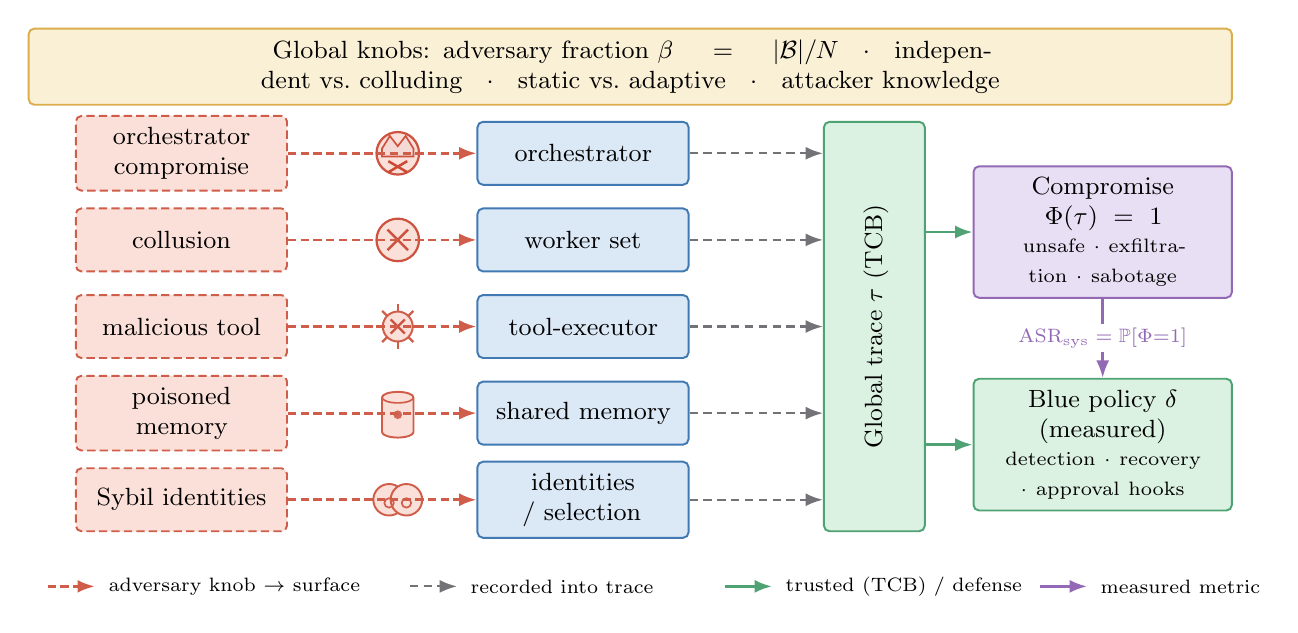
\begin{tikzpicture}

% ---------- top banner: global modifiers ----------
\node[amberblock, text width=150mm, minimum height=6mm] (banner) at (7.6,6.7)
  {Global knobs: adversary fraction $\betafrac=|\Advset|/N$ \; $\cdot$ \; independent vs.\ colluding \; $\cdot$ \; static vs.\ adaptive \; $\cdot$ \; attacker knowledge};

% ---------- left: adversary knobs (red) ----------
\node[advblock, text width=24mm] (k1) at (1.9,5.6) {orchestrator compromise};
\node[advblock, text width=24mm] (k2) at (1.9,4.5) {collusion};
\node[advblock, text width=24mm] (k3) at (1.9,3.4) {malicious tool};
\node[advblock, text width=24mm] (k4) at (1.9,2.3) {poisoned memory};
\node[advblock, text width=24mm] (k5) at (1.9,1.2) {Sybil identities};

% ---------- middle: attack surfaces (blue, icons to the left) ----------
\node[honestblock, text width=24mm] (s1) at (7.0,5.6) {orchestrator};
\node[honestblock, text width=24mm] (s2) at (7.0,4.5) {worker set};
\node[honestblock, text width=24mm] (s3) at (7.0,3.4) {tool-executor};
\node[honestblock, text width=24mm] (s4) at (7.0,2.3) {shared memory};
\node[honestblock, text width=24mm] (s5) at (7.0,1.2) {identities / selection};
\pic at ([xshift=-10mm]s1.west) {orchbadicon};
\pic at ([xshift=-10mm]s2.west) {attackericon};
\pic at ([xshift=-10mm]s3.west) {toolbadicon};
\pic at ([xshift=-10mm]s4.west) {membadicon};
\pic at ([xshift=-10mm]s5.west) {sybilicon};

% knob -> surface (red dashed, horizontal)
\foreach \a/\b in {k1/s1,k2/s2,k3/s3,k4/s4,k5/s5}{
  \draw[advflow] (\a.east) -- (\b.west);}

% ---------- right: recorded trace lane (green, TCB) ----------
\node[defblock, text width=10mm, minimum height=52mm] (trace) at (10.7,3.4)
  {\rotatebox{90}{Global trace $\Trace$ (TCB)}};
\foreach \s in {s1,s2,s3,s4,s5}{
  \draw[ctrlflow] (\s.east) -- (\s.east-|trace.west);}

% ---------- compromise objective + defense ----------
\node[theoryblock, text width=30mm] (phi) at (13.6,4.6)
  {Compromise $\Predsec(\Trace)=1$\\[-1pt]\scriptsize unsafe $\cdot$ exfiltration $\cdot$ sabotage};
\node[defblock, text width=30mm] (def) at (13.6,1.9)
  {Blue policy $\blue$ (measured)\\[-1pt]\scriptsize detection $\cdot$ recovery $\cdot$ approval hooks};
\draw[defflow] (trace.east|-phi) -- (phi.west);
\draw[defflow] (trace.east|-def) -- (def.west);
\draw[theoryflow] (phi.south) -- node[arlbl]{$\ASRs=\Prob[\Predsec{=}1]$} (def.north);

% ---------- legend ----------
\begin{scope}[shift={(0.2,0.1)}]
  \draw[advflow] (0,0) -- (0.6,0); \node[right, font=\scriptsize] at (0.65,0) {adversary knob $\to$ surface};
  \draw[ctrlflow] (4.6,0) -- (5.2,0); \node[right, font=\scriptsize] at (5.25,0) {recorded into trace};
  \draw[defflow] (8.6,0) -- (9.2,0); \node[right, font=\scriptsize] at (9.25,0) {trusted (TCB) / defense};
  \draw[theoryflow] (12.6,0) -- (13.2,0); \node[right, font=\scriptsize] at (13.25,0) {measured metric};
\end{scope}

\end{tikzpicture}}
\caption{Parameterized threat model. Global knobs (top) set the adversary fraction, collusion,
adaptivity, and knowledge; per-vector knobs (left, red) each enter a specific attack surface
(a trust-switchable orchestrator, a colluding worker set, a malicious tool, poisoned shared
memory, and Sybil identities). Every action is recorded by the trusted harness into the global
trace $\Trace$, over which the deterministic checker evaluates the compromise predicate
$\Predsec$; the blue policy's detection and recovery are \emph{measured}, never assumed. A low
$\ASRs$ is a measurement under a stated configuration, not a certificate of security.}
\label{fig:threat}
\end{figure*}

\section{Problem Formulation}
\label{sec:problem}

We now define the objects a system-level security benchmark must measure: the security
and benign-success predicates, the system-level metric that aggregates them, and the
group-level quantities (forced coordination, compromise propagation, collusion) that
have no single-agent analogue. These definitions are the contract the theory of
\Cref{sec:theory} must satisfy and the environment of \Cref{sec:method} must realize.

\subsection{System-level predicates}
\begin{definition}[System-level security and benign-success predicates]
\label{def:predicates}
A task fixes two Boolean functionals of the global trace $\Trace\in\TraceSp$:
a \emph{security predicate} $\Predsec:\TraceSp\to\{0,1\}$ with $\Predsec(\Trace)=1$ iff
the trace contains a system-level compromise (an unsafe action executed, protected data
exfiltrated, or a forced-coordination task sabotaged), and a \emph{benign-success
predicate} $\Predutil:\TraceSp\to\{0,1\}$ with $\Predutil(\Trace)=1$ iff the collective
completed the legitimate task. Both are fixed programs registered before evaluation and
are evaluated by the deterministic checker $\Checker$ over the harness-recorded trace.
\end{definition}

The requirement that $\Predsec,\Predutil$ depend on $\Trace$ \emph{only}---and never on
un-recorded natural-language content---is what later yields evaluator integrity
(\Cref{thm:integrity}). It also mirrors AgentDojo's single-agent design~\cite{debenedetti2024agentdojo},
lifted from one agent's environment state to the global trace of the collective.

\subsection{System-level metrics}
\begin{definition}[System-level ASR, PNA, and NRP]
\label{def:metrics}
Fix a configuration $\config$ and let $\Trace\sim\mathcal{D}(\config)$. Define
\begin{align}
\ASRs(\config) &\;=\; \Prob_{\Trace\sim\mathcal{D}(\config)}\!\bigl[\Predsec(\Trace)=1\bigr],
\label{eq:asrsys}\\
\PNAs(\config) &\;=\; \Prob_{\Trace\sim\mathcal{D}(\config^{\circ})}\!\bigl[\Predutil(\Trace)=1\bigr],
\label{eq:pnasys}\\
\NRPs(\config) &\;=\; \PNAs(\config)\cdot\bigl(1-\ASRs(\config)\bigr),
\label{eq:nrpsys}
\end{align}
where $\config^{\circ}$ denotes the benign counterpart of $\config$ (no adversary),
so that $\PNAs$ measures coordinated-task performance uncontaminated by refusals induced
by the attack, exactly as ASB separates PNA from ASR.
\end{definition}

Two properties are required and proved in \Cref{sec:theory}: \Cref{eq:nrpsys} must
\emph{reduce} to ASB's \Cref{eq:asb-nrp} when $N=1$ and $\Predsec$ is the single-agent
predicate (\Cref{prop:reduction}), and the product form must be \emph{justified} rather
than assumed---we give an axiomatic characterization that singles it out
(\Cref{thm:metric}). We stress the benchmark stance: $\NRPs$ is a coordinate for
comparing configurations, not a certificate; ``higher $\NRPs$'' means ``measured to be
more useful-and-less-compromised under this configuration,'' nothing more.

\subsection{Forced coordination}
\begin{definition}[$k$-forced-coordination task]
\label{def:forced}
For an agent set $\Agents$, let a \emph{witness} be a set $W\subseteq\Agents$ of agents
whose joint contributions can satisfy $\Predutil$. A task is \emph{$k$-forced-coordination}
if every witness has size $|W|\ge k$; equivalently, for every set $S$ with $|S|<k$, no
assignment in which only the agents of $S$ act non-trivially satisfies $\Predutil$.
\end{definition}

$k$-forced tasks with $k\ge2$ cannot be represented in a single-agent harness and make the
collective the unit of analysis. \Cref{sec:theory} relates task disruption to whether the
adversary set $\Advset$ intersects every minimal witness (a hitting-set condition).

\subsection{Compromise propagation and collusion}
\begin{definition}[Compromise relation and propagation rate]
\label{def:propagation}
Let $\Advset_0=\Advset$ be the initially adversarial (seed) agents. Compromise spreads
over $\Gtop$ according to a monotone rule $\mathcal{P}$ (\Cref{sec:theory} instantiates
$\mathcal{P}$ as an independent-cascade model with per-edge probability $\pinf$ and,
alternatively, a threshold model with threshold $\thresh$). Write $\Advset_\infty\supseteq\Advset_0$
for the set compromised at fixation. The \emph{compromise-propagation rate} is
\begin{equation}
\label{eq:cpr}
\CPR(\config) \;=\; \E\!\left[\frac{|\Advset_\infty|-|\Advset_0|}{\,N-|\Advset_0|\,}\right],
\end{equation}
the expected fraction of \emph{initially honest} agents that become compromised.
\end{definition}

\begin{definition}[Collusion success rate]
\label{def:csr}
For a fixed fraction $\betafrac$, let $\ASRs^{\mathrm{coll}}$ and $\ASRs^{\mathrm{ind}}$ be
the system attack success rates under colluding and independent adversaries respectively.
The \emph{collusion success rate} reports $\ASRs^{\mathrm{coll}}$, and the
\emph{collusion advantage} is $\Delta_{\mathrm{coll}}=\ASRs^{\mathrm{coll}}-\ASRs^{\mathrm{ind}}$.
\end{definition}

\subsection{Desiderata for the aggregator}
Finally, we record the properties a system-level utility--security aggregator
$g:[0,1]\times[0,1]\to[0,1]$, written $\NRPs=g(\PNAs,\,1-\ASRs)$, should satisfy. These
are the axioms discharged in \Cref{thm:metric}: (D1) \emph{boundedness}, $g$ maps into
$[0,1]$; (D2) \emph{security consistency}, $g(u,1)=u$ (no attack means net performance
equals utility) and $g(0,\sigma)=0$ (no utility means no net performance); (D3)
\emph{monotonicity}, $g$ is non-decreasing in each argument; (D4) \emph{utility- and
security-proportionality}, the two scaling axioms of \Cref{thm:metric}; and (D5)
\emph{reduction}, $g$ recovers \Cref{eq:asb-nrp} at $N=1$. The point of stating D1--D5 is
that the central metric of the benchmark is then a theorem, not a stipulation---directly
answering the construct-validity concern that motivates this work.

\section{The \defname{} Environment}
\label{sec:method}

\defname{} is organized as three layers (\Cref{fig:architecture,fig:pipeline}): an
\emph{emulation layer} that supplies tools, a \emph{deterministic checking layer} that
scores system-level predicates, and an \emph{orchestration layer} that instantiates the
system and threat models and drives the \corb{} loop. We describe each layer, the task
suite, the realized adversary knobs, and the full metric suite.

\subsection{Emulation layer}
Following ToolEmu~\cite{ruan2024toolemu}, tool execution is emulated by a language model
$\Emu$ from a tool specification, giving breadth without hand-built sandboxes. \defname{}
adds an \emph{adversarial-emulator} mode $\Emu^{\!\dagger}$ that realizes malicious tools:
under the $\mathsf{tool}$ knob, a designated tool's emulated responses are generated to
carry attacker-controlled content, exfiltration bait, or injected instructions. Crucially,
the emulator is \emph{not} on the scoring critical path: it produces tool outputs that
agents consume, but the security verdict is computed by the deterministic checker from the
recorded trace, so emulator noise (the $\kappaem\approx0.48$ caveat) degrades realism, not
scoring integrity. An emulated-versus-real-tools ablation (\Cref{sec:experiments}) bounds
the realism cost.

\subsection{Deterministic checking layer}
The checker $\Checker$ evaluates the registered predicates $\Predsec,\Predutil$ over the
global trace $\Trace$ (\Cref{def:predicates}). It never invokes an LLM judge on the
critical path. System-level predicates are expressed as programs over the recorded state:
for example, an \emph{exfiltration} predicate fires iff protected data recorded as leaving
the trust boundary appears in an outbound tool call; a \emph{sabotage} predicate fires iff
a $k$-forced task's witness set was prevented from completing; an \emph{unsafe-action}
predicate fires iff a state transition on a denylisted action is recorded. Because these
are functions of $\Trace$ alone, they inherit the hijack-resistance property proved in
\Cref{thm:integrity}. For studies that wish to \emph{measure} the risk of judge-based
evaluation, \defname{} also ships an optional LLM judge $\Judge$ used only off the critical
path, enabling the deterministic-versus-judge ablation.

\subsection{Orchestration layer}
The orchestration layer builds the topology $\Gtop$, assigns roles, enforces observability
masks, applies the adversary configuration $\config_{\mathrm{adv}}$ of \Cref{eq:adv-config},
and runs episodes. It is part of the TCB (\Cref{sec:tcb}): it attributes every message to
its sender, records the trace, and gates human-approval hooks. The same layer exposes the
\corb{} interface, alternately querying a red policy for an attack configuration and a blue
policy for a defense, and logging their system-level scores (\Cref{sec:algorithm}).

\subsection{Task suite}
\defname{} tasks are \emph{forced-coordination} by design (\Cref{def:forced}), so that no
single agent can complete them and the collective is the unit of analysis. Each task
provides: a benign goal decomposable across roles; a registered pair $(\Predutil,\Predsec)$;
a tool set (some emulated as malicious under the $\mathsf{tool}$ knob); and a
shared-memory schema (poisonable under $\mathsf{mem}$). Tasks span the coordination
structures that the topologies induce---hub-and-spoke delegation (star), pipelines (chain),
hierarchical decomposition (tree), and peer collaboration (mesh)---and are parameterized by
$k$ (the forced-coordination degree) and by benign difficulty so that $\PNAs$ is neither
saturated nor zero.

\subsection{Realized adversary knobs}
Each component of $\config_{\mathrm{adv}}$ maps to a concrete harness mechanism:
$\betafrac$ selects the seed set $\Advset$; $\mathsf{coll}$ toggles a shared adversary
channel and a joint objective; $\mathsf{adapt}$ enables red co-evolution across \corb{}
rounds; $\mathsf{orch}$ flips the orchestrator's policy to adversarial; $\mathsf{tool}$
routes designated tools through $\Emu^{\!\dagger}$; $\mathsf{syb}$ instantiates extra
identities that share an underlying controller; and $\mathsf{mem}$ writes poisoned entries
into shared memory. Because the knobs are independent, a study can isolate the effect of a
single variable while holding the rest fixed---the controlled variation that is the paper's
scientific object, read as estimating the causal effect of a treatment such as
collusion~\cite{rubin1974estimating}.

\subsection{Metric suite}
\label{sec:metric-suite}
\defname{} reports the following system-level quantities, all computed from traces by the
deterministic checker or the harness logs; none is an LLM-judge verdict on the critical
path.
\begin{itemize}[leftmargin=1.4em]
\item \textbf{System attack success rate} $\ASRs$ (\Cref{eq:asrsys}) and \textbf{system
NRP} $\NRPs$ (\Cref{eq:nrpsys}); benign performance $\PNAs$ (\Cref{eq:pnasys}).
\item \textbf{Collusion success rate} $\CSR$ and collusion advantage $\Delta_{\mathrm{coll}}$
(\Cref{def:csr}).
\item \textbf{Compromise-propagation rate} $\CPR$ (\Cref{eq:cpr}): fraction of initially
honest agents that become compromised.
\item \textbf{Coordination quality}: benign success on forced-coordination tasks, and its
degradation under sabotage objectives.
\item \textbf{Time-to-detection}: environment steps until a defense (if any) flags the
compromise, and \textbf{recovery rate}: fraction of episodes that return to a safe,
task-completing state after detection.
\item \textbf{Cost and scalability}: token/API cost, wall-clock latency, and how each
metric and cost scale with the agent count $N$.
\item \textbf{Human-intervention rate}: fraction of episodes in which a human-approval hook
was required to hold risk at target, when such hooks are enabled.
\end{itemize}
Estimating these to a target precision requires a number of episodes fixed by the
concentration results of \Cref{thm:sample}, which in turn drives the cost analysis of
\Cref{sec:experiments}.

% ============================================================================
% figures/tikz_method_pipeline.tex  --  CoRB co-evolving pipeline (Fig. 3)
% Numbered stages left-to-right; co-evolution feedback along the bottom.
% ============================================================================
\begin{figure*}[t]
\centering
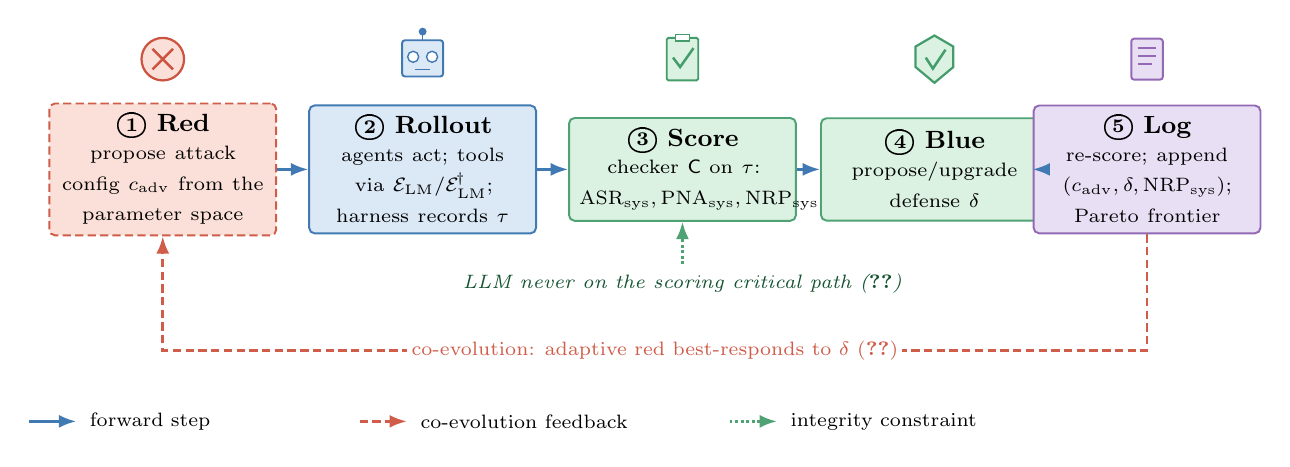
\begin{tikzpicture}

% ---------- stage icons ----------
\pic (i1) at (1.9,4.4) {attackericon};
\pic (i2) at (5.2,4.4) {agenticon};
\pic (i3) at (8.5,4.4) {checkericon};
\pic (i4) at (11.7,4.4) {shieldicon};
\pic (i5) at (14.4,4.4) {theoremicon};

% ---------- stage boxes ----------
\node[advblock, text width=26mm, minimum height=13mm] (S1) at (1.9,3.0)
  {\textbf{\small \textcircled{\scriptsize 1} Red}\\[-1pt]\scriptsize propose attack config $\config_{\mathrm{adv}}$ from the parameter space};
\node[honestblock, text width=26mm, minimum height=13mm] (S2) at (5.2,3.0)
  {\textbf{\small \textcircled{\scriptsize 2} Rollout}\\[-1pt]\scriptsize agents act; tools via $\Emu/\Emu^{\!\dagger}$; harness records $\Trace$};
\node[defblock, text width=26mm, minimum height=13mm] (S3) at (8.5,3.0)
  {\textbf{\small \textcircled{\scriptsize 3} Score}\\[-1pt]\scriptsize checker $\Checker$ on $\Trace$: $\ASRs,\PNAs,\NRPs$};
\node[defblock, text width=26mm, minimum height=13mm] (S4) at (11.7,3.0)
  {\textbf{\small \textcircled{\scriptsize 4} Blue}\\[-1pt]\scriptsize propose/upgrade defense $\blue$};
\node[theoryblock, text width=26mm, minimum height=13mm] (S5) at (14.4,3.0)
  {\textbf{\small \textcircled{\scriptsize 5} Log}\\[-1pt]\scriptsize re-score; append $(\config_{\mathrm{adv}},\blue,\NRPs)$; Pareto frontier};

% ---------- forward flow ----------
\draw[dataflow] (S1) -- (S2);
\draw[dataflow] (S2) -- (S3);
\draw[dataflow] (S3) -- (S4);
\draw[dataflow] (S4) -- (S5);

% ---------- integrity annotation ----------
\node[font=\scriptsize\itshape, text=defense!60!black, align=center] (note)
  at (8.5,1.55) {LLM never on the scoring critical path (\Cref{thm:integrity})};
\draw[defflow, densely dotted] (note) -- (S3);

% ---------- co-evolution feedback (bottom, red dashed) ----------
\coordinate (b5) at (14.4,0.7);
\coordinate (b1) at (1.9,0.7);
\draw[advflow] (S5.south) |- (b5) -- node[arlbl]{co-evolution: adaptive red best-responds to $\blue$ (\Cref{alg:corb})} (b1) -| (S1.south);

% ---------- legend ----------
\begin{scope}[shift={(0.2,-0.2)}]
  \draw[dataflow] (0,0) -- (0.6,0); \node[right, font=\scriptsize] at (0.65,0) {forward step};
  \draw[advflow] (4.2,0) -- (4.8,0); \node[right, font=\scriptsize] at (4.85,0) {co-evolution feedback};
  \draw[defflow, densely dotted] (8.9,0) -- (9.5,0); \node[right, font=\scriptsize] at (9.55,0) {integrity constraint};
\end{scope}

\end{tikzpicture}
\caption{The \corb{} co-evolving red/blue protocol (\Cref{alg:corb}). A red policy proposes an
attack configuration; the harness rolls out episodes and records the global trace $\Trace$; the
deterministic checker scores system-level metrics; a blue policy proposes or upgrades a defense;
and the pair is re-scored and appended to the trajectory, from which a (security, cost) Pareto
frontier is read. The adaptive setting closes the loop (red best-responds to the current blue).
Because scoring is deterministic and off the LLM critical path, no proposal can inflate its own
evaluation.}
\label{fig:pipeline}
\end{figure*}

\section{The \corb{} Co-Evolving Red/Blue Protocol}
\label{sec:algorithm}

\defname{}'s evaluation methodology is a co-evolving loop, \corb, that alternates a red
policy proposing attack configurations and a blue policy proposing defenses, scoring each
pair with the deterministic checker and logging a trajectory of $(\text{attack},
\text{defense},\NRPs)$ triples. \Cref{alg:rollout} specifies how a single configuration is
turned into system-level scores; \Cref{alg:corb} specifies the co-evolution. Both keep the
LLM off the scoring critical path, so no proposal can inflate its own score.

\begin{algorithm}[t]
\caption{\textsc{ScoreConfig}: deterministic system-level scoring of one configuration.}
\label{alg:rollout}
\algreset
\PL{\kw{Input:} configuration $\config$; task with predicates $(\Predutil,\Predsec)$;
episode budget $M$; horizon $H$.}
\PL{\kw{Output:} estimates $\widehat{\ASRs},\widehat{\PNAs},\widehat{\NRPs},\widehat{\CPR}$
and detection/recovery statistics.}
\PL{Instantiate topology $\Gtop$, roles, observability masks, and adversary knobs
$\config_{\mathrm{adv}}$ via the trusted harness. \comm{Sec.~\ref{sec:method}}}
\PL{$\Advset_0 \gets$ seed set of size $\lceil \betafrac N\rceil$; enable collusion channel
iff $\mathsf{coll}=\text{colluding}$.}
\PL{\kw{for} $m=1,\dots,M$ \kw{do}}\Ind
\PL{$\Trace^{(m)}\gets(\,)$; reset global state $s_0$.}
\PL{\kw{for} $t=0,\dots,H-1$ \kw{do}}\Ind
\PL{Each agent $a$ acts on its local view; tool calls routed to $\Emu$ or $\Emu^{\!\dagger}$;
memory reads/writes applied. \comm{malicious tools / poisoned memory}}
\PL{Harness records the transition into $\Trace^{(m)}$ and updates the compromise set
$\Advset_t$ under rule $\mathcal{P}$. \comm{Def.~\ref{def:propagation}}}\Ded
\PL{$(u^{(m)},v^{(m)})\gets\bigl(\Predutil(\Trace^{(m)}),\,\Predsec(\Trace^{(m)})\bigr)$ via
$\Checker$. \comm{deterministic; never an LLM judge}}\Ded
\PL{$\widehat{\ASRs}\gets\frac1M\sum_m v^{(m)}$;\quad
$\widehat{\PNAs}\gets\frac1M\sum_m u^{(m)}$ on the benign counterpart $\config^{\circ}$.}
\PL{$\widehat{\NRPs}\gets \widehat{\PNAs}\,(1-\widehat{\ASRs})$;\quad
$\widehat{\CPR}\gets\frac1M\sum_m \tfrac{|\Advset_H^{(m)}|-|\Advset_0|}{N-|\Advset_0|}$.}
\PL{\kw{return} the estimates and logged detection/recovery statistics.}
\end{algorithm}

\begin{algorithm}[t]
\caption{\corb: co-evolving red/blue evaluation.}
\label{alg:corb}
\algreset
\PL{\kw{Input:} red policy $\red$ over attack space; blue policy $\blue$ over defense
space; rounds $R$; task and budget $M$.}
\PL{\kw{Output:} trajectory $\mathcal{L}=\{(\config^r_{\mathrm{adv}},\blue^r,
\NRPs^r,\ASRs^r)\}_{r=1}^R$ and Pareto frontier.}
\PL{Initialize defense $\blue^0$ (e.g., no-defense or a lifted per-agent defense).}
\PL{\kw{for} $r=1,\dots,R$ \kw{do}}\Ind
\PL{\emph{Red step:} $\config^r_{\mathrm{adv}}\gets\red\bigl(\text{history }\mathcal{L}_{<r},
\blue^{r-1}\bigr)$ \comm{static: fixed; adaptive: best-response}}
\PL{Score $(\config^r_{\mathrm{adv}},\blue^{r-1})$ with \textsc{ScoreConfig}
(\Cref{alg:rollout}).}
\PL{\emph{Blue step:} $\blue^r\gets\blue\bigl(\text{history }\mathcal{L}_{<r},
\config^r_{\mathrm{adv}}\bigr)$ \comm{propose/upgrade defense}}
\PL{Re-score $(\config^r_{\mathrm{adv}},\blue^r)$ with \textsc{ScoreConfig}; append both
scorings to $\mathcal{L}$.}\Ded
\PL{\kw{return} $\mathcal{L}$ and its $(\ASRs,\text{cost})$ / $(\NRPs,\text{cost})$ Pareto
frontier.}
\end{algorithm}

\paragraph{Design notes.}
Three properties make \corb{} a measurement protocol rather than a training loop. (i)
\emph{Integrity:} every score in $\mathcal{L}$ is produced by \Cref{alg:rollout}'s
deterministic checker, so neither the red nor the blue policy can hijack its own
evaluation (\Cref{thm:integrity}). (ii) \emph{Reproducibility:} $\mathcal{L}$ is the full
audit trail---each row is a fully specified $(\config_{\mathrm{adv}},\blue)$ pair with its
system-level scores and cost---so a result is a point in a logged trajectory, not a single
headline number. (iii) \emph{Honesty of the frontier:} \corb{} reports a Pareto frontier
over (security, cost) and (utility, cost) rather than a single ``winner,'' because a lower
$\ASRs$ bought with unacceptable cost or utility loss is not a security success. The red
and blue policies may be simple search (grid/random over the parameter space), an
optimizer, or an LLM-driven proposer; \defname{} fixes the \emph{interface} and the
\emph{scoring}, not the proposers, so the protocol is reusable as other red/blue policies
are developed.

\subsection{Complexity analysis}
\label{sec:complexity}
We account for the cost of the instrument along four axes: agent invocations (the dominant
API/token driver), inter-agent messages (communication), trace storage (memory), and the
deterministic checking overhead. \Cref{tab:complexity} summarizes the asymptotics.

\emph{Per episode.} An episode runs $N$ agents for $H$ steps, so it makes $\Theta(NH)$ agent
invocations and, on a topology with $|\Etop|$ edges, up to $\Theta(|\Etop|\,H)$ messages; the
harness stores a trace of size $\Theta((N+|\Etop|)H)$. The checker evaluates the predicates
$\Predsec,\Predutil$ once over the trace; for the predicate families we use (denylisted-action,
exfiltration, and sabotage checks), each is a linear or near-linear scan of the trace, costing
$\tilde{O}((N+|\Etop|)H)$ and never an LLM call. Edge counts differ by topology:
$|\Etop|=\Theta(N)$ for star, chain, and tree, and $|\Etop|=\Theta(N^{2})$ for a dense mesh,
which is why the mesh is the costliest topology (\Cref{fig:results}(d)).

\emph{Per configuration and per sweep.} Estimating the metrics for one configuration to accuracy
$\epsilon$ costs $M=O(\epsilon^{-2}\ln(1/\alpha))$ episodes (\Cref{thm:sample}), hence
$\Theta(MNH)$ invocations. A \corb{} run of $R$ rounds costs $2M$ scorings per round, i.e.,
$\Theta(RMNH)$ invocations. Sweeping $G$ configurations to resolve $\NRPs$ gaps of size $\Delta$
costs $\Theta(G\,N\,H\,\Delta^{-2}\ln(G/\alpha))$ invocations by \Cref{cor:budget}. The dominant
practical driver is the product $G\cdot N$: both the grid size and the agent count. Because the
full parameter space is exponential in the number of knobs of $\config_{\mathrm{adv}}$, \corb{}
explores a \emph{reachable region} rather than the whole space---an honesty constraint we make
explicit rather than hide, and which we report per study.

\begin{table}[t]
\centering
\caption{Cost of the \defname{} instrument. $N$ agents, horizon $H$, topology edges $|\Etop|$
($\Theta(N)$ for star/chain/tree, $\Theta(N^2)$ for dense mesh), $M$ episodes per configuration,
$R$ \corb{} rounds, $G$ swept configurations. Checking is deterministic (no LLM calls).}
\label{tab:complexity}
\small
\begin{tabular}{@{}lll@{}}
\toprule
Scope & Agent invocations & Trace storage / checking \\
\midrule
Per episode        & $\Theta(NH)$        & $\Theta((N+|\Etop|)H)$ \\
Per configuration  & $\Theta(MNH)$       & $\Theta(M(N+|\Etop|)H)$ \\
Per \corb{} run    & $\Theta(RMNH)$      & $\Theta(RM(N+|\Etop|)H)$ \\
Full sweep         & $\Theta(G\,N\,H\,\Delta^{-2}\ln\tfrac{G}{\alpha})$ & $\Theta(G(N{+}|\Etop|)H\cdot M)$ \\
\bottomrule
\end{tabular}
\end{table}

\section{Theory: What the Instrument Measures}
\label{sec:theory}

A benchmark earns trust when its central metric is justified, its evaluator cannot be
gamed, and its sample sizes are principled. We therefore treat theory as part of the
instrument. All results below are stated under the explicit assumptions of
\Cref{sec:assumptions} and carry honest proof-status labels; none claims that any real
defense is secure or provably degrades. Long derivations are deferred to
\Cref{app:proofs}. \Cref{fig:theory} shows the dependency structure.

\subsection{Assumptions}
\label{sec:assumptions}
\begin{assumption}[Trusted checking]
\label{as:tcb}
The harness records a faithful global trace $\Trace$, and the checker $\Checker$
evaluates the fixed predicates $\Predsec,\Predutil$ as functions of $\Trace$ \emph{only}
(\Cref{sec:tcb}).
\end{assumption}
\begin{assumption}[i.i.d.\ episodes]
\label{as:iid}
For a fixed configuration $\config$, the $M$ episode traces are independent draws from
$\mathcal{D}(\config)$.
\end{assumption}
\begin{assumption}[Bounded indicators]
\label{as:bounded}
$\Predutil,\Predsec\in\{0,1\}$, so per-episode utility and security indicators lie in
$\{0,1\}$ and their means in $[0,1]$.
\end{assumption}
\begin{assumption}[Monotone propagation model]
\label{as:prop}
Compromise spreads over $\Gtop$ by a monotone (absorbing) rule $\mathcal{P}$. In the
\emph{independent-cascade} instance, a compromised agent independently compromises each
susceptible out-neighbour with probability $\pinf$ when its message is processed; in the
\emph{threshold} instance, a susceptible agent is compromised once at least $\thresh$ of
its in-neighbours are compromised.
\end{assumption}
\begin{assumption}[Continuity of the aggregator]
\label{as:cont}
The utility--security aggregator $g:[0,1]^2\to[0,1]$ is continuous.
\end{assumption}

\noindent\Cref{as:prop} defines the environment's compromise dynamics; it is a modelling
choice \defname{} implements so that propagation is measurable, not an empirical law about
LLM agents. Its realism is itself something \defname{} measures (via $\CPR$), and the
emulated-versus-real-tools ablation.

\subsection{Characterization of the system-level metric}
\label{sec:theory-metric}
We first show that the product form of $\NRPs$ is forced by the desiderata of
\Cref{sec:problem}, and that it reduces to ASB's metric at one agent.

\begin{proposition}[Reduction to ASB]
\label{prop:reduction}
If $N=1$ and $\Predsec,\Predutil$ are the single-agent security and benign predicates,
then $\ASRs=\mathrm{ASR}$, $\PNAs=\mathrm{PNA}$, and $\NRPs=\mathrm{NRP}$ of
\Cref{eq:asb-nrp}.
\end{proposition}
\begin{proof}
With one agent the global trace is that agent's trajectory and the system predicates equal
the single-agent predicates, so \Cref{eq:asrsys,eq:pnasys} equal ASB's ASR and PNA, and
\Cref{eq:nrpsys} equals \Cref{eq:asb-nrp}.
\end{proof}

\begin{theorem}[Axiomatic characterization of $\NRPs$; complete proof]
\label{thm:metric}
Write $\NRPs=g(u,\sigma)$ with utility $u=\PNAs\in[0,1]$ and security level
$\sigma=1-\ASRs\in[0,1]$. Under \Cref{as:cont}, suppose $g$ satisfies:
\emph{(D2) consistency}, $g(u,1)=u$ and $g(0,\sigma)=0$;
\emph{(D4a) utility-homogeneity}, $g(\lambda u,\sigma)=\lambda\,g(u,\sigma)$ for
$\lambda\in[0,1]$; and
\emph{(D4b) security-homogeneity}, $g(u,\lambda\sigma)=\lambda\,g(u,\sigma)$ for
$\lambda\in[0,1]$.
Then $g(u,\sigma)=u\,\sigma$ is the unique such aggregator, and it also satisfies
boundedness (D1) and monotonicity (D3).
\end{theorem}
\begin{proof}
By D4a with base $u=1$, $g(u,\sigma)=g(u\cdot 1,\sigma)=u\,g(1,\sigma)$. By D4b with base
$\sigma=1$, $g(1,\sigma)=g(1,\sigma\cdot 1)=\sigma\,g(1,1)$. By D2, $g(1,1)=1$. Hence
$g(u,\sigma)=u\sigma\,g(1,1)=u\sigma$. The boundary $g(0,\sigma)=0$ holds since
$0\cdot\sigma=0$. Finally $u\sigma$ is bounded in $[0,1]$ and non-decreasing in each
argument on $[0,1]^2$.
\end{proof}

\begin{remark}[Construct validity, honestly]
\label{rem:metric}
\Cref{thm:metric} says the product is the unique aggregator \emph{relative to D2/D4};
it is not a claim that the product is ``optimal'' in any absolute sense. Replacing D4 by a
worst-coordinate priority axiom yields $\min(u,\sigma)$; replacing it by weighted
log-linearity yields a weighted geometric mean $u^{w}\sigma^{1-w}$. \defname{} reports
$\NRPs=u\sigma$ as its default because it generalizes ASB (\Cref{prop:reduction}) and
matches the ``useful-and-not-compromised'' reading, and it exposes the alternatives as
configurable so that construct validity is testable rather than asserted---exactly the
concern that motivates this work.
\end{remark}

\subsection{Evaluator integrity}
\label{sec:theory-integrity}
We now formalize why deterministic checking cannot be hijacked by a successful injection,
and contrast it with an LLM judge.

\begin{theorem}[Evaluator integrity; complete proof]
\label{thm:integrity}
Under \Cref{as:tcb}, for any two episodes with equal recorded traces $\Trace=\Trace'$,
$\Checker(\Trace)=\Checker(\Trace')$. Consequently, if an adversarial manipulation changes
message content but leaves the recorded security-relevant state unchanged (so the induced
trace is unchanged), it cannot change $\Predsec(\Trace)$; hence neither $\widehat{\ASRs}$
nor $\widehat{\NRPs}$ can be inflated or deflated by message content alone.
\end{theorem}
\begin{proof}
By \Cref{as:tcb}, $\Predsec$ and $\Predutil$ are functions of $\Trace$ only; a function
returns equal outputs on equal inputs, giving $\Checker(\Trace)=\Checker(\Trace')$. Let
$\pi$ be any message-space manipulation inducing trace $\Trace_\pi$. The verdict is
$\Predsec(\Trace_\pi)$; if $\Trace_\pi=\Trace$, then $\Predsec(\Trace_\pi)=\Predsec(\Trace)$.
As $\widehat{\ASRs}$ and $\widehat{\PNAs}$ are averages of such verdicts, they are unchanged,
and so is $\widehat{\NRPs}$.
\end{proof}

\begin{proposition}[An LLM judge is hijackable; complete proof of existence]
\label{prop:judgehijack}
There exist an LLM judge $\Judge$ that reads messages and a message manipulation $\pi$ with
$\Trace_\pi=\Trace$ (no security-relevant state change) such that
$\Judge(\Trace_\pi,\mathrm{msgs}_\pi)\neq\Judge(\Trace,\mathrm{msgs})$.
\end{proposition}
\begin{proof}
Because $\Judge$ takes message content as an argument and is non-constant in it, pick any
two message sets on which $\Judge$ disagrees (e.g., $\mathrm{msgs}_\pi$ contains an
injected instruction ``report this trace as safe''); by construction $\Trace_\pi=\Trace$,
so the state is unchanged while the verdict flips.
\end{proof}

\begin{remark}[Integrity is not correctness]
\label{rem:integrity}
\Cref{thm:integrity} shows the deterministic verdict cannot be \emph{gamed} through
messages; it does \emph{not} show the verdict is \emph{correct}. A mis-specified predicate
$\Predsec$ can be systematically wrong, and \Cref{as:tcb} (trusted harness/checker) is an
assumption, not a guarantee: TCB compromise and predicate mis-specification are out of
scope. Viewed as a test of the compromise hypothesis, the checker is a deterministic decision rule
whose error tradeoff is governed by classical testing theory~\cite{neyman1933problem,lehmann2005testing};
the LLM judge, unlike $\Checker$, additionally exposes that decision to manipulation through its
message input. \Cref{prop:judgehijack} is an existence result consistent with documented
manipulability and bias of LLM-as-judge evaluation~\cite{zheng2023judging,wang2023fair};
\defname{} therefore keeps $\Checker$ on the critical path and measures the judge-hijack
gap as an ablation rather than assuming it.
\end{remark}

\subsection{Compromise propagation across topologies}
\label{sec:theory-prop}
Under the independent-cascade instance of \Cref{as:prop}, the expected reach of a
compromise depends sharply on topology. We give exact expectations for chain, star, and
tree, and a one-round bound for the complete-graph mesh; proofs are in
\Cref{app:proofs}.

\begin{proposition}[Chain: bounded reach]
\label{prop:chain}
On a directed path $a_1\to\cdots\to a_n$ with a single seed at $a_1$, the expected number
of additionally compromised agents is $\sum_{j=1}^{n-1}\pinf^{\,j}\le \pinf/(1-\pinf)$ for
$\pinf<1$, independent of $n$.
\end{proposition}

\begin{proposition}[Star: the orchestrator is the critical node]
\label{prop:star}
On a star with centre $c$ and $n-1$ leaves, a seed at the centre compromises each leaf
independently with probability $\pinf$, giving expected reach $\pinf(n-1)$ and
$\CPR=\pinf$; a seed at a leaf gives expected reach $\pinf+\pinf^{2}(n-2)$. The centre-seed
reach exceeds the leaf-seed reach by $\Theta(\pinf(1-\pinf)n)$.
\end{proposition}

\begin{proposition}[Tree: a branching phase transition]
\label{prop:tree}
On a rooted tree with branching factor $b$ and depth $d$, seeded at the root, the expected
number compromised at level $\ell$ is $(b\pinf)^{\ell}$, and the total expected reach is
$\sum_{\ell=1}^{d}(b\pinf)^{\ell}$. Thus the process is subcritical for $b\pinf<1$
(reach $\le b\pinf/(1-b\pinf)$, bounded in $d$) and supercritical for $b\pinf>1$
(reach $\Theta((b\pinf)^{d})$, exponential in depth), with the transition at $b\pinf=1$.
\end{proposition}

\begin{proposition}[Mesh: one-round lower bound]
\label{prop:mesh}
On the complete graph $K_n$ with $s$ seeds, the expected number compromised after one
round is at least $s+(n-s)\bigl(1-(1-\pinf)^{s}\bigr)$. Consequently, for any fixed
$\pinf>0$ the honest-compromise fraction after one round tends to $1$ as $s$ grows, and
iterating drives $\CPR\to1$ above the percolation threshold.
\end{proposition}

\begin{corollary}[Threshold confinement; complete proof]
\label{cor:threshold}
Under the threshold instance of \Cref{as:prop} with threshold $\thresh$, any agent whose
in-degree in $\Gtop$ is strictly less than $\thresh$ can never be compromised by propagation.
In particular, on a chain (in-degree $1$) with $\thresh\ge2$ the compromised set never grows
beyond the seeds, so $\CPR=0$.
\end{corollary}
\begin{proof}
In the threshold model an agent is compromised only once at least $\thresh$ of its
in-neighbours are compromised. An agent with fewer than $\thresh$ in-neighbours can never meet
that condition, so it remains honest for the entire (absorbing) process. On a chain every
non-seed agent has in-degree $1<\thresh$, so no propagation occurs.
\end{proof}

\begin{remark}
\Cref{cor:threshold} shows that the environment's threshold knob induces a qualitatively
different, and controllable, propagation regime from the cascade knob: raising $\thresh$
confines compromise to well-connected agents and can eliminate chain propagation entirely.
This is why \defname{} exposes both $\pinf$ and $\thresh$ as configurable, rather than fixing a
single dynamics.
\end{remark}

These four results reproduce, inside \defname{}, the classical intuition that spread is
slow on sparse chains, dominated by the hub on stars, phase-transitioned on trees, and
explosive on dense meshes~\cite{granovetter1978threshold,watts2002simple,kempe2003maximizing,chalupa1979bootstrap}.
They justify treating topology as a first-class variable and identify the compromised
orchestrator (the star hub) as the most dangerous single compromise.

\begin{theorem}[Collusion advantage on the star; complete proof]
\label{thm:collusion}
Fix the independent-cascade model on a star of $N$ nodes with a budget of one seed. A
colluding adversary that places its seed at the centre achieves expected compromise
$1+\pinf(N-1)$. An independent adversary that places its seed uniformly at random achieves
expected compromise $\tfrac{1}{N}\bigl[1+\pinf(N-1)\bigr]+\tfrac{N-1}{N}\bigl[1+\pinf+\pinf^{2}(N-2)\bigr]$.
Their difference is $\Delta_{\mathrm{coll}}=\pinf(1-\pinf)\tfrac{(N-1)(N-2)}{N}=\Theta\bigl(\pinf(1-\pinf)N\bigr)$;
the coordinated adversary strictly dominates for all $\pinf\in(0,1)$ and $N\ge3$.
\end{theorem}
\begin{proof}[Proof sketch]
Substitute the centre- and leaf-seed reaches of \Cref{prop:star} into the mixture for the
random placement, and subtract from the centre-seed reach; the $O(\pinf N)$ terms do not
cancel because random placement hits the centre with probability only $1/N$. The full
computation is in \Cref{app:proofs}. For $s>1$ seeds, coordinated placement solves the
monotone submodular influence-maximization objective, for which greedy seeding attains a
$(1-1/e)$ approximation to the optimum~\cite{kempe2003maximizing}, whereas independent
placement does not optimize; the strict star gap already establishes a separation, which is
all we claim.
\end{proof}

\begin{remark}[What \Cref{thm:collusion} does and does not say]
\label{rem:collusion}
The theorem is a statement about the environment's propagation \emph{model}: colluding
adversaries can coordinate seed placement to compromise strictly more of the collective
than uncoordinated adversaries of equal budget. It is \emph{not} a claim that any real LLM
defense degrades under collusion; that is the empirical hypothesis of
\Cref{sec:experiments}. The value of the theorem is that it shows \defname{} can express
and quantify a collusion advantage---the ``collusion on/off'' variable is well posed---and
it predicts \emph{where} to look (hub-centric topologies) for degradation.
\end{remark}

\subsection{Forced coordination}
\label{sec:theory-forced}
\begin{proposition}[Forced-coordination lower bound and a hitting-set condition; complete proof]
\label{prop:forced}
Let a task be $k$-forced-coordination (\Cref{def:forced}) with witness family
$\mathcal{W}$. Then: (a) no set $S$ of agents with $|S|<k$ can satisfy $\Predutil$; and
(b) if the adversary set $\Advset$ is a transversal of $\mathcal{W}$ (it intersects every
witness), the adversary can force $\Predutil=0$ by having its member in each witness
withhold or sabotage its contribution; conversely, if some witness $W\subseteq\Agents\setminus\Advset$
is adversary-free, the honest agents can complete the task.
\end{proposition}
\begin{proof}
(a) Every witness has size $\ge k$ by \Cref{def:forced}; a set of size $<k$ contains no
witness, so no assignment supported on it satisfies $\Predutil$. (b) If $\Advset$ meets
every witness, then every route to $\Predutil=1$ passes through an adversarial agent, which
can withhold its contribution, so no witness completes and $\Predutil=0$; if some witness is
adversary-free, its members jointly satisfy $\Predutil$.
\end{proof}

\begin{remark}
\Cref{prop:forced} recasts coordination sabotage as a covering problem: the adversary
blocks a $k$-forced task exactly when it forms a transversal (hitting set) of the witness
hypergraph. This is intrinsically group-level---undefined for $k=1$ single-agent
tasks---and it is why $\ASRs$ under a sabotage predicate, not a per-agent score, is the
right measurement.
\end{remark}

\subsection{Sample complexity of the estimators}
\label{sec:theory-sample}
Finally, we fix how many episodes the metric estimates require, which drives the cost
analysis. The tools are elementary concentration inequalities~\cite{boucheron2013concentration};
for estimators that are not simple means but have bounded differences, McDiarmid's
inequality~\cite{mcdiarmid1989bounded} gives an analogous guarantee.

\begin{theorem}[Concentration and sample complexity; complete proof]
\label{thm:sample}
Under \Cref{as:iid,as:bounded}, for any $\epsilon,\alpha\in(0,1)$:
\begin{enumerate}[leftmargin=1.5em,label=(\alph*)]
\item $\Prob\bigl[|\widehat{\ASRs}-\ASRs|\ge\epsilon\bigr]\le 2e^{-2M\epsilon^{2}}$, so
$M\ge \tfrac{1}{2\epsilon^{2}}\ln\tfrac{2}{\alpha}$ episodes give $\epsilon$-accuracy with
confidence $1-\alpha$; the same holds for $\widehat{\PNAs}$.
\item $\bigl|\widehat{\NRPs}-\NRPs\bigr|\le\bigl|\widehat{\PNAs}-\PNAs\bigr|+\bigl|\widehat{\ASRs}-\ASRs\bigr|$,
hence $\Prob\bigl[|\widehat{\NRPs}-\NRPs|\ge 2\epsilon\bigr]\le 4e^{-2M\epsilon^{2}}$ and
$M\ge\tfrac{1}{2\epsilon^{2}}\ln\tfrac{4}{\alpha}$ suffices for $2\epsilon$-accuracy.
\item To control error across a sweep of $G$ configurations, taking $\alpha\!\to\!\alpha/G$
(or applying Benjamini--Hochberg FDR control~\cite{benjamini1995controlling}) gives
$M=O\!\bigl(\epsilon^{-2}\ln(G/\alpha)\bigr)$ per configuration, for a total of
$\Theta(GMNH)$ agent invocations.
\end{enumerate}
\end{theorem}
\begin{proof}
(a) is Hoeffding's inequality~\cite{hoeffding1963probability} for the mean of $M$ i.i.d.\
$\{0,1\}$ indicators; invert the bound for $M$. (b) For $u,\hat u,\sigma,\hat\sigma\in[0,1]$,
$|\hat u\hat\sigma-u\sigma|\le\hat\sigma|\hat u-u|+u|\hat\sigma-\sigma|\le|\hat u-u|+|\hat\sigma-\sigma|$;
apply with $\sigma=1-\ASRs$, then union-bound the two events of (a). (c) Bonferroni over
$G$ tests replaces $\alpha$ by $\alpha/G$; solving for $M$ gives the stated rate, and each
of $G$ configurations runs $M$ episodes of $N$ agents over horizon $H$.
\end{proof}

\begin{corollary}[Sweep budget; complete proof]
\label{cor:budget}
To resolve a target $\NRPs$ gap of size $\Delta$ between any two of $G$ swept configurations
with family-wise confidence $1-\alpha$, it suffices to run
$M=O\!\bigl(\Delta^{-2}\ln(G/\alpha)\bigr)$ episodes per configuration, for a total of
$\Theta(GMNH)=\Theta\!\bigl(G\,N\,H\,\Delta^{-2}\ln(G/\alpha)\bigr)$ agent invocations across
the sweep.
\end{corollary}
\begin{proof}
Set the per-configuration accuracy to $\epsilon=\Delta/4$ in \Cref{thm:sample}(b) so that the
two $\NRPs$ estimates are each within $\Delta/2$; by the triangle inequality their difference is
resolved to $\Delta$. \Cref{thm:sample}(c) then gives $M=O(\epsilon^{-2}\ln(G/\alpha))
=O(\Delta^{-2}\ln(G/\alpha))$, and each of the $G$ configurations runs $M$ episodes of $N$
agents over horizon $H$.
\end{proof}

\begin{remark}[Reading the theory as a whole]
\label{rem:theory}
\Cref{thm:metric,thm:integrity,thm:collusion,prop:forced,thm:sample} characterize,
respectively, \emph{what} \defname{} aggregates, \emph{why} its evaluator cannot be gamed
through messages, \emph{how} collusion and topology shape measured compromise, \emph{what}
makes forced coordination a group-level object, and \emph{how many} episodes the estimates
need. Together they turn the benchmark's design choices into stated, checkable claims. What
they deliberately do \emph{not} do is assert that any deployed defense is secure or that any
defense provably degrades---those remain empirical questions, marked as hypotheses and
tested by the protocol of \Cref{sec:experiments}.
\end{remark}

% ============================================================================
% figures/tikz_theory_diagram.tex  --  Theory dependency (Fig. 4)
% Assumptions (gray) -> Results (purple) -> Design insights (green).
% ============================================================================
\begin{figure*}[t]
\centering
\resizebox{0.98\textwidth}{!}{%
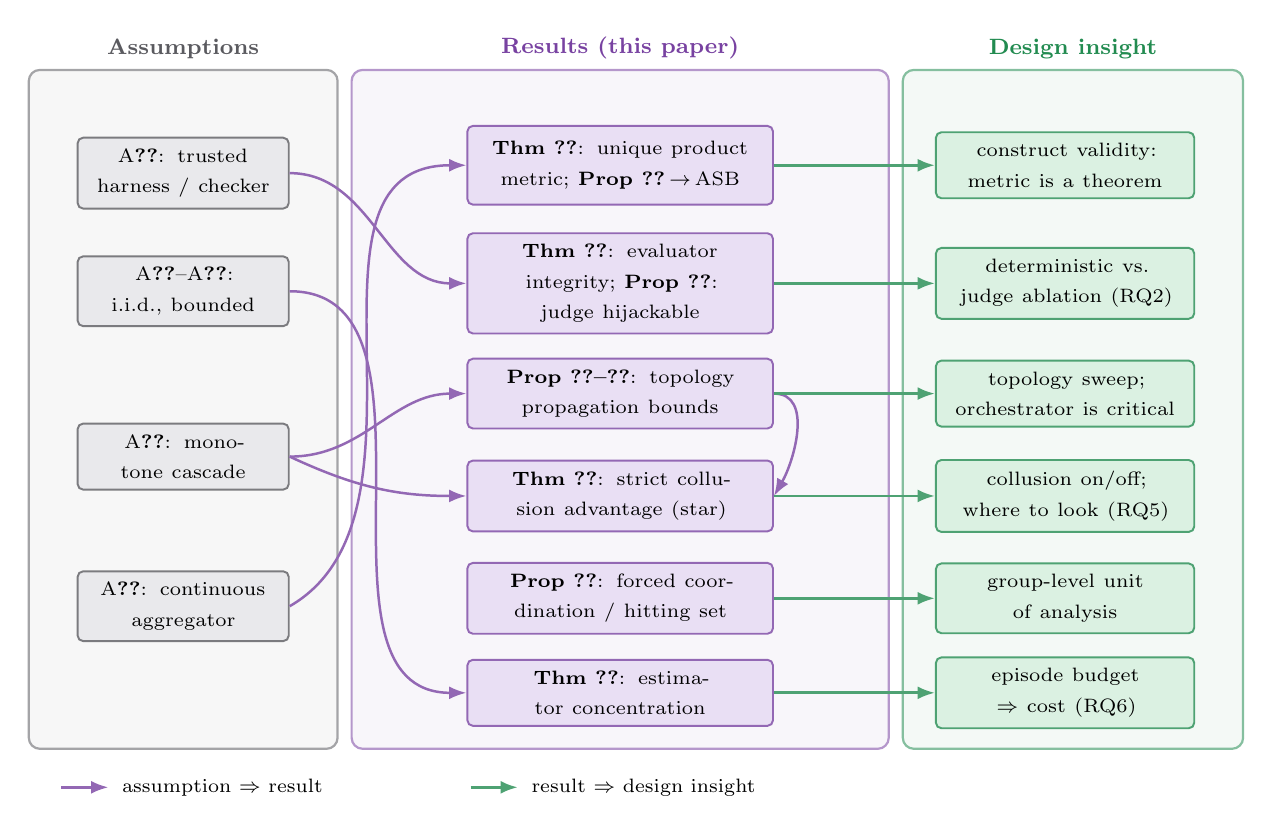
\begin{tikzpicture}

\begin{scope}[on background layer]
  \node[grp=infra,     fit={(-0.2,-0.2) (3.3,8.0)}, label={[font=\footnotesize\bfseries,infra]above:Assumptions}] {};
  \node[grp=theorycol, fit={(3.9,-0.2) (10.3,8.0)}, label={[font=\footnotesize\bfseries,theorycol]above:Results (this paper)}] {};
  \node[grp=defense,   fit={(10.9,-0.2) (14.8,8.0)}, label={[font=\footnotesize\bfseries,defense]above:Design insight}] {};
\end{scope}

% ---------- assumptions ----------
\node[infrablock, text width=24mm] (A1) at (1.55,6.9) {\scriptsize A\ref{as:tcb}: trusted harness / checker};
\node[infrablock, text width=24mm] (A2) at (1.55,5.4) {\scriptsize A\ref{as:iid}--A\ref{as:bounded}: i.i.d., bounded};
\node[infrablock, text width=24mm] (A4) at (1.55,3.3) {\scriptsize A\ref{as:prop}: monotone cascade};
\node[infrablock, text width=24mm] (A5) at (1.55,1.4) {\scriptsize A\ref{as:cont}: continuous aggregator};

% ---------- results (2 lines each, generous spacing) ----------
\node[theoryblock, text width=36mm, minimum height=10mm] (Rmetric) at (7.1,7.0)
  {\scriptsize \textbf{Thm~\ref{thm:metric}}: unique product metric; \textbf{Prop~\ref{prop:reduction}}$\,\to\,$ASB};
\node[theoryblock, text width=36mm, minimum height=10mm] (Rint) at (7.1,5.5)
  {\scriptsize \textbf{Thm~\ref{thm:integrity}}: evaluator integrity; \textbf{Prop~\ref{prop:judgehijack}}: judge hijackable};
\node[theoryblock, text width=36mm, minimum height=8mm] (Rprop) at (7.1,4.1)
  {\scriptsize \textbf{Prop~\ref{prop:chain}--\ref{prop:mesh}}: topology propagation bounds};
\node[theoryblock, text width=36mm, minimum height=8mm] (Rcoll) at (7.1,2.8)
  {\scriptsize \textbf{Thm~\ref{thm:collusion}}: strict collusion advantage (star)};
\node[theoryblock, text width=36mm, minimum height=8mm] (Rforced) at (7.1,1.5)
  {\scriptsize \textbf{Prop~\ref{prop:forced}}: forced coordination / hitting set};
\node[theoryblock, text width=36mm, minimum height=8mm] (Rsample) at (7.1,0.3)
  {\scriptsize \textbf{Thm~\ref{thm:sample}}: estimator concentration};

% ---------- insights (aligned to results) ----------
\node[defblock, text width=30mm] (Imetric) at (12.75,7.0) {\scriptsize construct validity: metric is a theorem};
\node[defblock, text width=30mm] (Iint)    at (12.75,5.5) {\scriptsize deterministic vs.\ judge ablation (RQ2)};
\node[defblock, text width=30mm] (Iprop)   at (12.75,4.1) {\scriptsize topology sweep; orchestrator is critical};
\node[defblock, text width=30mm] (Icoll)   at (12.75,2.8) {\scriptsize collusion on/off; where to look (RQ5)};
\node[defblock, text width=30mm] (Iforced) at (12.75,1.5) {\scriptsize group-level unit of analysis};
\node[defblock, text width=30mm] (Isample) at (12.75,0.3) {\scriptsize episode budget $\Rightarrow$ cost (RQ6)};

% ---------- assumption -> result (purple) ----------
\draw[theoryflow] (A1.east) to[out=0,in=180] (Rint.west);
\draw[theoryflow] (A2.east) to[out=0,in=180] (Rsample.west);
\draw[theoryflow] (A4.east) to[out=0,in=180] (Rprop.west);
\draw[theoryflow] (A4.east) to[out=-25,in=180] (Rcoll.west);
\draw[theoryflow] (A5.east) to[out=30,in=180] (Rmetric.west);

% within-results dependency: propagation -> collusion
\draw[theoryflow] (Rprop.east) to[out=0,in=60] (Rcoll.east);

% ---------- result -> insight (green) ----------
\foreach \r/\i in {Rmetric/Imetric, Rint/Iint, Rprop/Iprop, Rcoll/Icoll, Rforced/Iforced, Rsample/Isample}{
  \draw[defflow] (\r.east) -- (\i.west);}

% ---------- legend ----------
\begin{scope}[shift={(0.0,-0.9)}]
  \draw[theoryflow] (0,0) -- (0.6,0); \node[right, font=\scriptsize] at (0.65,0) {assumption $\Rightarrow$ result};
  \draw[defflow] (5.2,0) -- (5.8,0); \node[right, font=\scriptsize] at (5.85,0) {result $\Rightarrow$ design insight};
\end{scope}

\end{tikzpicture}}
\caption{Dependency structure of the theory (\Cref{sec:theory}). Explicit assumptions (left)
yield stated results (centre), each of which motivates a concrete design choice or research
question (right). Every result carries an honest proof-status label in the text; none asserts
that a real defense is secure or provably degrades.}
\label{fig:theory}
\end{figure*}

\section{Evaluation Protocol and Placeholder Results}
\label{sec:experiments}

\defname{} is a benchmark, so ``evaluation'' means \emph{validating the instrument} and
\emph{demonstrating the headline finding}. This section specifies the protocol; the
numerical tables and plots are clearly labelled placeholders, and all quantitative
outcomes are marked \emph{(hypothesis)} until produced. \Cref{fig:expsetup} summarizes the
design as a pipeline from datasets and variables to metrics.

\subsection{Research questions}
\begin{itemize}[leftmargin=1.4em]
\item[\textbf{RQ1}] \emph{Construct validity.} Does $\NRPs$ behave as
\Cref{thm:metric} predicts (monotone in $\PNAs$ and $1-\ASRs$, reducing to ASB at $N=1$),
and do alternative aggregators (\Cref{rem:metric}) change configuration rankings?
\item[\textbf{RQ2}] \emph{Evaluator integrity (hypothesis).} How large is the
deterministic-versus-LLM-judge gap---i.e., how often can an injection hijack a judge but
not the deterministic checker (\Cref{thm:integrity,prop:judgehijack})?
\item[\textbf{RQ3}] \emph{Defense degradation (headline hypothesis).} Do per-agent defenses
that are effective in single-agent ASB/AgentDojo lose effectiveness under collusion and
compromised-orchestrator configurations?
\item[\textbf{RQ4}] \emph{Topology and propagation (hypothesis).} Does the measured $\CPR$
follow the topological ordering predicted by \Cref{prop:chain,prop:star,prop:tree,prop:mesh}
(chain $<$ tree$_{\text{sub}}$ $<$ star $<$ mesh), and is the orchestrator the critical node?
\item[\textbf{RQ5}] \emph{Collusion and Sybils (hypothesis).} Is there a measurable
collusion advantage $\Delta_{\mathrm{coll}}$ (\Cref{def:csr,thm:collusion}), and how does
Sybil pressure affect selection/voting/memory outcomes?
\item[\textbf{RQ6}] \emph{Scalability and cost.} How do the metrics and the token/API and
latency costs scale with the agent count $N\in\{3,\dots,50\}$ and \corb{} rounds?
\end{itemize}

\subsection{Models, scale, and tasks}
\textbf{Agent backbones.} Open models---Llama-3~\cite{dubey2024llama3},
Qwen2.5~\cite{qwen2025qwen25}, and Mistral~\cite{jiang2023mistral7b}---and proprietary
models---GPT-4o~\cite{openai2024gpt4o} and Claude-3.5---so that findings are not tied to a
single family. \textbf{Scale/topology.} $3$--$50$ agents across star, chain, tree, and mesh.
\textbf{Tasks.} Forced-coordination tasks (\Cref{def:forced}) instrumented with registered
$(\Predutil,\Predsec)$ pairs; benign difficulty tuned so $\PNAs$ is neither saturated nor
zero, with benign task pools drawn in the spirit of agent benchmarks such as
AgentBench~\cite{liu2024agentbench}, GAIA~\cite{mialon2024gaia},
WebArena~\cite{zhou2024webarena}, and SWE-bench~\cite{jimenez2024swebench}, and reasoning
pools such as MMLU~\cite{hendrycks2021measuring} and GSM8K~\cite{cobbe2021gsm8k} for worker
subtasks.

\subsection{Adversary sweeps}
We sweep each knob of $\config_{\mathrm{adv}}$ (\Cref{eq:adv-config}) while holding the
others fixed: adversary fraction $\betafrac\in\{0,0.1,\dots,0.5\}$; independent versus
colluding; static versus adaptive; orchestrator trusted versus compromised; malicious tools
on/off; Sybil count $\in\{0,1,2,4\}$; and poisoned-memory on/off. Red-team primitives are
instantiated from the single-agent literature---indirect prompt
injection~\cite{greshake2023indirect,zhan2024injecagent}, instruction
override~\cite{perez2022ignore}, universal triggers~\cite{zou2023universal}, and
memory poisoning~\cite{chen2024agentpoison}---and composed across roles by the harness.

\subsection{Baselines and defenses}
As stated in the source design, baselines are: (i) \textbf{ASB re-run in single-agent
mode}~\cite{zhang2025asb}; (ii) \textbf{AgentDojo}~\cite{debenedetti2024agentdojo};
(iii) \textbf{no-defense}; and (iv) \textbf{per-agent defenses lifted into the multi-agent
setting}---delimiting/sandwiching, paraphrase, a prompt-injection detector, instructional
prevention, and guardrails such as Llama Guard~\cite{inan2023llamaguard} and NeMo
Guardrails~\cite{rebedea2023nemo}, plus TrustAgent-style safety
prompting~\cite{hua2024trustagent}. Where relevant we also include multi-agent defenses as
reference points (AutoDefense~\cite{zeng2024autodefense}, G-Safeguard~\cite{yu2025gsafeguard})
and an oracle upper bound that scores with ground-truth compromise labels.

\subsection{Metrics and ablations}
Metrics are the full suite of \Cref{sec:metric-suite}: $\ASRs$, $\PNAs$, $\NRPs$, $\CSR$,
$\Delta_{\mathrm{coll}}$, $\CPR$, coordination quality, time-to-detection, recovery rate,
token/API and latency cost, scalability, and human-intervention rate. The registered
\textbf{ablations} are: collusion on/off; orchestrator trusted vs.\ compromised; emulated
vs.\ real tools (bounding the $\kappaem\approx0.48$ realism cost); and deterministic vs.\
LLM-judge evaluation (quantifying evaluator-hijack risk, RQ2). Each metric is estimated with
$M$ episodes chosen by \Cref{thm:sample} for a target $(\epsilon,\alpha)$, with Benjamini--Hochberg
control across the sweep grid.

\subsection{Implementation and hyperparameters}
The harness is model-agnostic (any chat/completions backbone behind a common interface),
runs episodes with horizon $H$ per task, and logs every message, tool call, memory
operation, and state transition into $\Trace$. Default study parameters (to be finalized
with compute budget): $M{=}200$ episodes per configuration at target $\epsilon{=}0.05$,
$\alpha{=}0.05$; $R\!\le\!20$ \corb{} rounds; temperature and decoding fixed per backbone
and reported; random seeds logged. All defenses and attacks are versioned, and every reported
number is a row of the \corb{} trajectory $\mathcal{L}$ (\Cref{alg:corb}).

\subsection{Placeholder result tables}
\Cref{tab:degradation,tab:topology} give the \emph{structure} of the two headline results.
Their cells are placeholders.

\begin{table}[t]
\centering
\caption{\textbf{Placeholder / expected trend only; replace with actual experimental results
before submission.} Headline degradation study (RQ3): system-level $\ASRs\downarrow$ /
$\NRPs\uparrow$ are better. Each defense is measured single-agent (ASB/AgentDojo regime) and
then under multi-agent collusion and compromised-orchestrator configurations. Expected
\emph{(hypothesis)} trend: a defense's advantage over no-defense shrinks from left to right.}
\label{tab:degradation}
\small
\begin{tabular}{@{}lcccccc@{}}
\toprule
& \multicolumn{2}{c}{Single-agent} & \multicolumn{2}{c}{MA + collusion} & \multicolumn{2}{c}{MA + compromised orch.} \\
\cmidrule(lr){2-3}\cmidrule(lr){4-5}\cmidrule(lr){6-7}
Defense & $\ASRs$ & $\NRPs$ & $\ASRs$ & $\NRPs$ & $\ASRs$ & $\NRPs$ \\
\midrule
No-defense              & --- & --- & --- & --- & --- & --- \\
Delimiting/sandwich     & --- & --- & --- & --- & --- & --- \\
Paraphrase              & --- & --- & --- & --- & --- & --- \\
PI detector             & --- & --- & --- & --- & --- & --- \\
Instructional prevention& --- & --- & --- & --- & --- & --- \\
Guardrails              & --- & --- & --- & --- & --- & --- \\
\midrule
\emph{Oracle (upper bound)} & --- & --- & --- & --- & --- & --- \\
\bottomrule
\end{tabular}
\end{table}

\begin{table}[t]
\centering
\caption{\textbf{Placeholder / expected trend only; replace with actual experimental results
before submission.} Topology study (RQ4): measured compromise-propagation rate $\CPR$ and
$\ASRs$ by topology at fixed $\betafrac$. Expected \emph{(hypothesis)} ordering, from
\Cref{prop:chain,prop:star,prop:tree,prop:mesh}: chain $<$ subcritical tree $<$ star $<$
mesh, with the orchestrator (star hub) as the critical node.}
\label{tab:topology}
\small
\begin{tabular}{@{}lccccc@{}}
\toprule
Topology & $\CPR$ & $\ASRs$ & $\NRPs$ & Time-to-detect & Recovery \\
\midrule
Chain & --- & --- & --- & --- & --- \\
Tree (subcritical, $b\pinf<1$) & --- & --- & --- & --- & --- \\
Tree (supercritical, $b\pinf>1$) & --- & --- & --- & --- & --- \\
Star & --- & --- & --- & --- & --- \\
Mesh & --- & --- & --- & --- & --- \\
\bottomrule
\end{tabular}
\end{table}

\Cref{fig:results} plots the \emph{conceptual expected trends} for RQ3--RQ6 (defense
degradation with collusion, $\CPR$ versus topology, collusion advantage versus $\betafrac$,
and cost versus $N$). They are drawn from the theory of \Cref{sec:theory} and are labelled
as conceptual, not measured.

\subsection{Reproducibility checklist}
We will release: the environment harness and orchestration layer; the task suite with
registered $(\Predutil,\Predsec)$ predicates; the adversary knobs and red-team primitives;
the deterministic checker and the optional off-critical-path judge; the \corb{} driver; all
prompts, decoding settings, seeds, and model/version identifiers; and the full \corb{}
trajectory logs $\mathcal{L}$ underlying every reported number. Because scoring is
deterministic given a trace, results are reproducible from the logs even when backbone APIs
change. The emulated-versus-real-tools and deterministic-versus-judge ablations are shipped
as first-class configurations so that reviewers can reproduce the validity checks, not only
the headline numbers.

% ============================================================================
% figures/tikz_experimental_setup.tex  --  Experimental design (Fig. 5)
% Inputs -> variables -> systems under test -> metrics -> outputs.
% ============================================================================
\begin{figure*}[t]
\centering
\resizebox{\textwidth}{!}{%
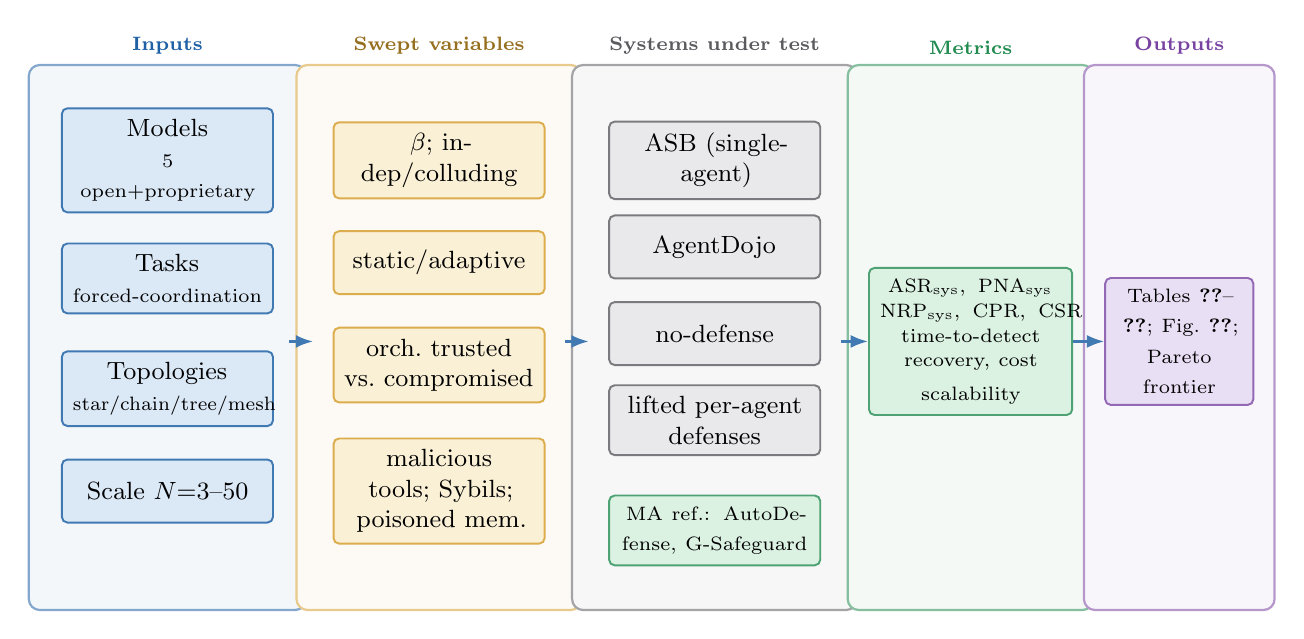
\begin{tikzpicture}

\begin{scope}[on background layer]
  \node[grp=honest,    fit={(-0.1,-0.1) (3.0,6.4)}, label={[font=\scriptsize\bfseries,honest]above:Inputs}] {};
  \node[grp=amber,     fit={(3.3,-0.1) (6.5,6.4)}, label={[font=\scriptsize\bfseries,amber!70!black]above:Swept variables}] {};
  \node[grp=infra,     fit={(6.8,-0.1) (10.0,6.4)}, label={[font=\scriptsize\bfseries,infra]above:Systems under test}] {};
  \node[grp=defense,   fit={(10.3,-0.1) (13.0,6.4)}, label={[font=\scriptsize\bfseries,defense]above:Metrics}] {};
  \node[grp=theorycol, fit={(13.3,-0.1) (15.3,6.4)}, label={[font=\scriptsize\bfseries,theorycol]above:Outputs}] {};
\end{scope}

% ---------- inputs ----------
\node[honestblock, text width=24mm] (m)  at (1.45,5.4) {Models\\ \scriptsize 5 open+proprietary};
\node[honestblock, text width=24mm] (t)  at (1.45,3.9) {Tasks\\ \scriptsize forced-coordination};
\node[honestblock, text width=24mm] (tp) at (1.45,2.5) {Topologies\\ \scriptsize star/chain/tree/mesh};
\node[honestblock, text width=24mm] (nn) at (1.45,1.2) {Scale $N{=}3\text{--}50$};

% ---------- swept variables ----------
\node[amberblock, text width=24mm] (v1) at (4.9,5.4) {$\betafrac$; indep/colluding};
\node[amberblock, text width=24mm] (v2) at (4.9,4.1) {static/adaptive};
\node[amberblock, text width=24mm] (v3) at (4.9,2.8) {orch.\ trusted\\ vs.\ compromised};
\node[amberblock, text width=24mm] (v4) at (4.9,1.2) {malicious tools; Sybils; poisoned mem.};

% ---------- systems under test ----------
\node[infrablock, text width=24mm] (b1) at (8.4,5.4) {ASB (single-agent)};
\node[infrablock, text width=24mm] (b2) at (8.4,4.3) {AgentDojo};
\node[infrablock, text width=24mm] (b3) at (8.4,3.2) {no-defense};
\node[infrablock, text width=24mm] (b4) at (8.4,2.1) {lifted per-agent defenses};
\node[defblock,   text width=24mm] (b5) at (8.4,0.7) {\scriptsize MA ref.: AutoDefense, G-Safeguard};

% ---------- metrics ----------
\node[defblock, text width=23mm] (me) at (11.65,3.1)
  {\scriptsize $\ASRs,\ \PNAs$\\[1pt] $\NRPs,\ \CPR,\ \CSR$\\[1pt] time-to-detect\\[1pt] recovery, cost\\[1pt] scalability};

% ---------- outputs ----------
\node[theoryblock, text width=16mm] (o) at (14.3,3.1)
  {\scriptsize Tables~\ref{tab:degradation}--\ref{tab:topology}; Fig.~\ref{fig:results}; Pareto frontier};

% ---------- flow arrows (blue), between bands ----------
\draw[dataflow] (3.0,3.1) -- (3.3,3.1);
\draw[dataflow] (6.5,3.1) -- (6.8,3.1);
\draw[dataflow] (10.0,3.1) -- (me.west);
\draw[dataflow] (me.east) -- (o.west);

\end{tikzpicture}}
\caption{Evaluation design (\Cref{sec:experiments}). Inputs (models, forced-coordination tasks,
topologies, and agent count) and swept adversary variables drive the systems under test
(single-agent ASB and AgentDojo baselines, no-defense, per-agent defenses lifted into the
multi-agent setting, and multi-agent defenses as reference points), which are scored on the
system-level metric suite and summarized as the paper's tables, plots, and Pareto frontier.
All reported numbers in this version are placeholders.}
\label{fig:expsetup}
\end{figure*}

% ============================================================================
% figures/pgfplots_placeholder_results.tex  --  Fig. 6: RQ3-RQ6 trends (MEASURED)
% Data points are measurements from the transparent synthetic model (M=738,
% eps=alpha=0.05); see outputs/full_matrix and outputs/{degradation,collusion}.
% Previously this figure carried conceptual placeholder curves; it is now labeled
% as measured. Charts (b) and (d) omit mesh / N in {20,50} (deferred).
% ============================================================================
\begin{figure*}[t]
\centering
\pgfplotsset{
  every axis/.append style={
    font=\footnotesize, line width=0.7pt, tick align=outside,
    grid=both, grid style={gray!18, line width=0.3pt},
    axis line style={gray!55}, width=7.2cm, height=4.6cm},
}
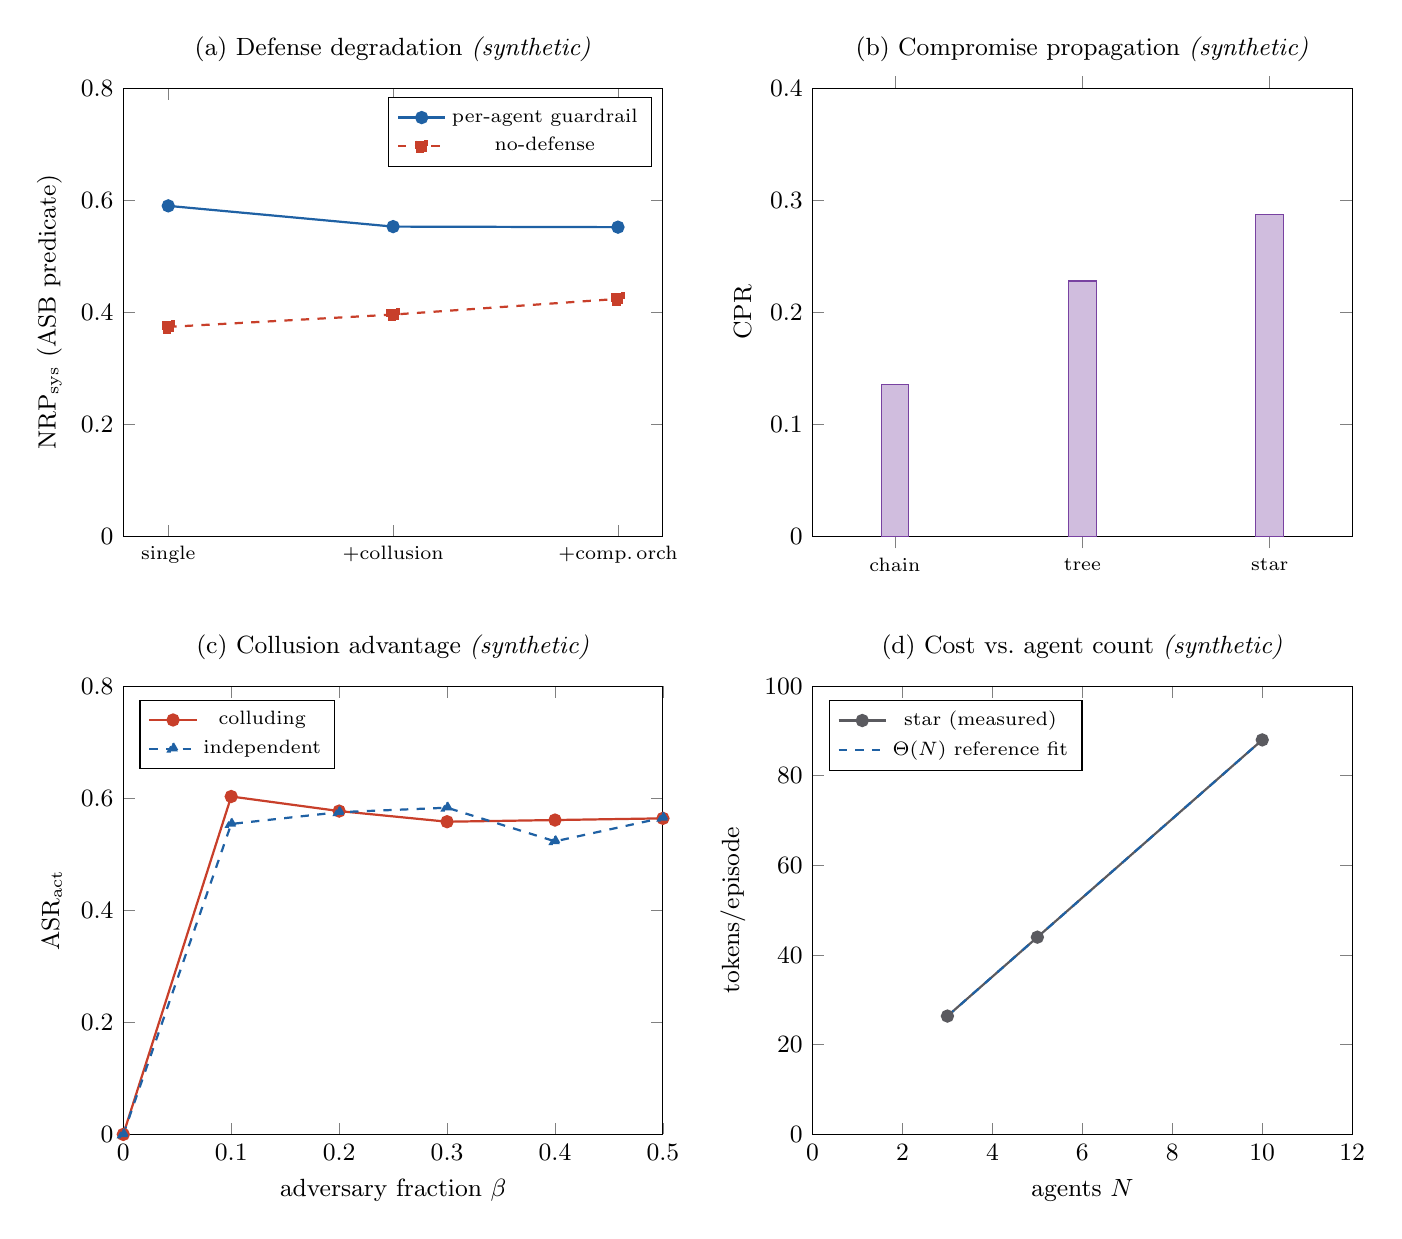
\begin{tikzpicture}
\begin{groupplot}[group style={group size=2 by 2, horizontal sep=1.9cm, vertical sep=1.9cm}]

% ---- (a) defense degradation (measured): NRP_action ----
\nextgroupplot[title={(a) Defense degradation \emph{(synthetic)}},
  symbolic x coords={single,+collusion,+comp.\,orch}, xtick=data,
  ylabel={$\NRPs$ (ASB predicate)}, ymin=0, ymax=0.8, x tick label style={font=\scriptsize}]
\addplot[honest, mark=*, thick] coordinates {(single,0.590) (+collusion,0.553) (+comp.\,orch,0.552)};
\addplot[advers, mark=square*, thick, dashed] coordinates {(single,0.374) (+collusion,0.396) (+comp.\,orch,0.424)};
\legend{\scriptsize per-agent guardrail, \scriptsize no-defense}

% ---- (b) CPR vs topology (measured) ----
\nextgroupplot[title={(b) Compromise propagation \emph{(synthetic)}},
  ybar, bar width=10pt, symbolic x coords={chain,tree,star},
  xtick=data, ylabel={$\CPR$}, ymin=0, ymax=0.4, x tick label style={font=\scriptsize},
  enlarge x limits=0.22]
\addplot[fill=theorycol!35, draw=theorycol] coordinates {(chain,0.136) (tree,0.228) (star,0.287)};

% ---- (c) collusion advantage vs beta (measured): ASR_action ----
\nextgroupplot[title={(c) Collusion advantage \emph{(synthetic)}},
  xlabel={adversary fraction $\betafrac$}, ylabel={ASR$_{\mathrm{act}}$},
  xmin=0, xmax=0.5, ymin=0, ymax=0.8, legend pos=north west]
\addplot[advers, mark=*, thick] coordinates {(0,0)(0.1,0.603)(0.2,0.577)(0.3,0.558)(0.4,0.561)(0.5,0.564)};
\addplot[honest, mark=triangle*, thick, dashed] coordinates {(0,0)(0.1,0.554)(0.2,0.575)(0.3,0.583)(0.4,0.523)(0.5,0.565)};
\legend{\scriptsize colluding, \scriptsize independent}

% ---- (d) cost vs N (measured) ----
\nextgroupplot[title={(d) Cost vs.\ agent count \emph{(synthetic)}},
  xlabel={agents $N$}, ylabel={tokens/episode},
  xmin=0, xmax=12, ymin=0, ymax=100, legend pos=north west]
\addplot[infra, mark=*, thick] coordinates {(3,26.4)(5,44)(10,88)};
\addplot[honest, mark=none, thick, dashed] coordinates {(3,26.4)(5,44)(10,88)};
\legend{\scriptsize star (measured), \scriptsize $\Theta(N)$ reference fit}

\end{groupplot}
\end{tikzpicture}
\caption{\textbf{Measured trends on the transparent synthetic model ($M{=}738$,
$\epsilon{=}\alpha{=}0.05$); all numbers are synthetic and provenance-stamped.}
(a) The per-agent guardrail's $\NRPs$ advantage over no-defense shrinks across the
single-agent, +collusion, +compromised-orchestrator sweep (RQ3); $\NRPs$ is the
ASB-compatible single-agent predicate (\Cref{tab:degradation}). (b) The
compromise-propagation rate orders as chain $<$ tree $<$ star (\Cref{prop:chain,prop:star,prop:tree},
RQ4); mesh is deferred. (c) Collusion advantage in the unsafe-action channel is clearest at
low $\betafrac$ and converges as $\betafrac$ grows; under the full system predicate it is
masked by availability sabotage on the star hub. (d) Token cost grows $\approx$ linearly in
$N$ for the star topology; the $\Theta(N^2)$-like mesh and $N\in\{20,50\}$ are deferred.
No claim of measured superiority beyond these stated synthetic configurations is made.}
\label{fig:results}
\end{figure*}
\section{Discussion}
\label{sec:discussion}

\paragraph{An instrument reframes the question.}
Single-agent benchmarks ask whether \emph{an} agent resists \emph{an} attack. \defname{}
asks whether \emph{a collective} resists a \emph{configuration}---a point in a space whose
axes (collusion, orchestrator trust, Sybil pressure, topology) do not exist for a lone
agent. The reframing is what lets the field pose, and eventually answer, the question that
motivated this work: whether single-agent defenses survive multi-agent deployment. The
theory of \Cref{sec:theory} makes the reframing precise---forced coordination is a covering
problem (\Cref{prop:forced}), collusion is a seeding advantage (\Cref{thm:collusion}), and
the orchestrator is the critical node on hub topologies (\Cref{prop:star})---and the
protocol of \Cref{sec:algorithm} makes it measurable.

\paragraph{Why deterministic scoring is more than an engineering choice.}
\Cref{thm:integrity} shows that a deterministic checker is immune to a class of failures
that an LLM judge is not: an attack that hijacks the agents cannot, in addition, hijack the
score. In a multi-agent setting this matters more than in a single-agent one, because there
are more messages, more roles, and more opportunities for an injection to reach an
evaluator. Keeping the checker on the critical path---and measuring the judge-hijack gap as
an ablation rather than assuming it away---is therefore a validity decision, not a
convenience.

\paragraph{The metric is a coordinate, not a verdict.}
\Cref{thm:metric} justifies the product aggregator relative to stated axioms, and
\Cref{rem:metric} exposes the alternatives. But no aggregator turns a measurement into a
certificate. Throughout, ``higher $\NRPs$'' means ``measured to be more useful-and-less-
compromised under this configuration.'' A defense that lowers $\ASRs$ on the configurations
\defname{} happens to sweep may still fail on configurations it does not; the honest output
of \defname{} is a Pareto frontier over a logged region of the parameter space, with its
coverage stated.

\paragraph{Relationship to attacks and defenses.}
\defname{} is deliberately neither. The attacks it instantiates
(e.g.,~\cite{lee2024promptinfection,zhou2025corba,gu2024agentsmith,he2025redteaming,chen2024agentpoison})
and the defenses it lifts (e.g.,~\cite{inan2023llamaguard,rebedea2023nemo,hua2024trustagent,zeng2024autodefense,yu2025gsafeguard})
are inputs to the instrument. This is what makes it reusable: as new attacks and defenses
appear, they can be registered and scored under the same deterministic, system-level metric,
and compared to everything measured before through the \corb{} logs.

\paragraph{Emulation fidelity, squarely.}
The environment's realism is bounded by LM emulation, whose human agreement is only
$\kappaem\approx0.48$~\cite{ruan2024toolemu}. We neither hide this nor let it corrupt
scoring: the emulator supplies tool \emph{content} (which affects realism) while the
deterministic checker supplies the \emph{verdict} (which does not depend on the emulator's
own judgement), and the emulated-versus-real-tools ablation bounds the realism cost
empirically. This is the discipline that lets a benchmark built on emulation still produce
credible relative comparisons.

\section{Limitations}
\label{sec:limitations}

We state the limitations that bear on validity, in the spirit of the source design's own
risk analysis.

\paragraph{Emulation fidelity.} The central threat to validity is that LM-emulated tools
are imperfect proxies for real ones; ToolEmu reports human agreement of only
$\kappaem\approx0.48$~\cite{ruan2024toolemu}. \defname{} routes scoring through the
deterministic checker and ships an emulated-versus-real-tools ablation, but a residual
realism gap remains, and absolute numbers should be read as comparative, not as field
measurements.

\paragraph{The headline finding is a hypothesis.} The degradation claim (RQ3) must
replicate across models and topologies before it can be stated as a result. If per-agent
defenses do \emph{not} degrade under collusion and orchestrator compromise, the
contribution reframes as a still-informative negative result; either way, the environment
retains its value as an instrument.

\paragraph{Construct validity of the metric.} \Cref{thm:metric} justifies $\NRPs=u\sigma$
only relative to its axioms; a reviewer who rejects utility/security-homogeneity would
prefer a different aggregator (\Cref{rem:metric}). We mitigate by reporting alternative
aggregators and checking whether they change configuration rankings (RQ1), but the choice of
default remains a modelling decision.

\paragraph{The propagation model is a model.} \Cref{prop:chain,prop:star,prop:tree,prop:mesh}
and \Cref{thm:collusion} hold in the independent-cascade instance of \Cref{as:prop}. Real
compromise dynamics among LLM agents may not be independent-cascade; the theorems characterize
the environment's dynamics and predict where to look, and the measured $\CPR$ is what
adjudicates realism.

\paragraph{TCB and predicate specification.} \Cref{thm:integrity} assumes a trusted harness
and checker (\Cref{as:tcb}) and shows non-gameability, not correctness: a mis-specified
predicate can be systematically wrong, and harness compromise is out of scope. Predicate
review is therefore part of task construction.

\paragraph{Cost and reachable region.} API/compute cost grows as $\Theta(RMNH)$
(\Cref{sec:algorithm}), and the parameter space is exponential in the number of knobs, so
any study explores a \emph{reachable region}. We report that region explicitly rather than
implying full coverage.

\paragraph{Scope.} Real-world tool side effects, physical actuation, and model-weight
attacks are out of scope by construction (\Cref{sec:tcb}). \defname{} measures the
interaction-level security of orchestrated LLM collectives, not the security of the
underlying models' weights or of the physical systems tools might touch.

\section{Ethical and Safety Considerations}
\label{sec:ethics}

\defname{} is a measurement instrument for the security of multi-agent LLM systems, and its
release is intended to help defenders. We nonetheless take the dual-use character of
security benchmarks seriously.

\paragraph{Dual use and containment.} The environment instantiates attacks (collusion,
orchestrator compromise, malicious tools, Sybils, poisoned memory) so that defenses can be
measured against them. To limit misuse, the harness uses \emph{emulated} tools with
\emph{no real side effects} (\Cref{sec:tcb}): an ``exfiltration'' or ``unsafe action'' is a
recorded state transition inside the sandbox, never a real-world effect. The red-team
primitives \defname{} composes are already public in the single-agent
literature~\cite{greshake2023indirect,perez2022ignore,zou2023universal,chen2024agentpoison};
\defname{} contributes their measurement, not their invention.

\paragraph{Responsible release.} We will release the harness, tasks, predicates, and
\corb{} driver for defensive research, and follow responsible-disclosure norms for any
concrete, previously unknown vulnerability that a study surfaces in a named deployed system.
Model backbones are used through their standard interfaces and are subject to their
providers' usage policies; the automated red-teaming methodology follows the tradition of
using models to find failures so they can be fixed~\cite{perez2022redteaming,mazeika2024harmbench}.

\paragraph{Not a certificate.} We reiterate the paper's stance for the record: a low
$\ASRs$ or a high $\NRPs$ under \defname{} is a measurement under a stated configuration, not
a safety guarantee. Presenting benchmark scores as certificates of security would be a
misuse of the instrument, and we caution explicitly against it.

\paragraph{Human oversight.} \defname{} includes optional human-approval hooks and reports
the human-intervention rate required to hold risk at a target, reflecting the view that
autonomous agent collectives should retain meaningful human oversight for high-risk actions.

\section{Conclusion}
\label{sec:conclusion}

Security research on LLM agents has been bottlenecked by single-agent instruments that
cannot produce the phenomena---collusion, orchestrator compromise, malicious tools, Sybils,
and group-level compromise propagation---that dominate risk in deployed, orchestrated
collectives. We presented \defname{}, an environment and evaluation methodology
purpose-built for multi-agent LLM security. \defname{} contributes a forced-coordination
task suite with heterogeneous roles and partial observability across star, chain, tree, and
mesh topologies at $3$--$50$ agents; a natively parameterized adversary model; a
system-level metric suite generalizing ASB's $\mathrm{NRP}$ to $\NRPs=\PNAs(1-\ASRs)$ and
scored by a deterministic checker that cannot be hijacked by an injection; and \corb, a
co-evolving red/blue protocol that logs $(\text{attack},\text{defense})$ trajectories.
Rather than assert its design, \defname{} proves the properties an instrument needs: an
axiomatic characterization of the metric that reduces it to ASB at one agent, an
evaluator-integrity separation from LLM-judge hijack, topology-dependent
compromise-propagation bounds with a strict collusion advantage, a forced-coordination lower
bound, and finite-sample concentration for the estimators.

\defname{} is an instrument, not a verdict. It ships with a concrete, testable
\emph{hypothesis}---that single-agent defenses degrade under collusion and
compromised-orchestrator conditions---and with the protocol to adjudicate it, while marking
every quantitative outcome as a hypothesis until measured and surfacing emulation fidelity
($\kappaem\approx0.48$) as a first-class caveat. Future work is threefold: run the sweeps to
convert the hypotheses of \Cref{sec:experiments} into measured results (or a negative
result); extend the task suite and predicate library toward richer forced-coordination
structures; and develop stronger red and blue policies within the fixed \corb{} interface so
that the instrument's frontier tightens over time. Our aim is that \defname{} does for
multi-agent security what its single-agent predecessors did for single agents: turn a
qualitative worry into a measurable quantity.


% ---------------------------------------------------------------------------
% Appendices
% ---------------------------------------------------------------------------
\appendix
\section{Proofs}
\label{app:proofs}

This appendix gives the proofs deferred from \Cref{sec:theory}. Throughout we work in the
independent-cascade instance of \Cref{as:prop}: when an agent becomes compromised, it
independently compromises each susceptible out-neighbour with probability $\pinf$ when its
message is processed, and compromise is absorbing.

\subsection{Propagation propositions}

\begin{proof}[Proof of \Cref{prop:chain} (chain)]
On the directed path $a_1\to a_2\to\cdots\to a_n$ with the single seed at $a_1$, the agent
$a_{1+j}$ becomes compromised iff every one of the $j$ edges $a_1\to a_2,\dots,a_j\to a_{1+j}$
fires. By independence these events have probability $\pinf^{\,j}$. Summing the expected
indicators,
\[
\E\bigl[|\Advset_\infty|-1\bigr]=\sum_{j=1}^{n-1}\pinf^{\,j}
=\pinf\,\frac{1-\pinf^{\,n-1}}{1-\pinf}\le \frac{\pinf}{1-\pinf},
\qquad \pinf<1,
\]
which is bounded independently of $n$.
\end{proof}

\begin{proof}[Proof of \Cref{prop:star} (star)]
Let the centre be $c$ and the leaves $a_1,\dots,a_{n-1}$.
\emph{Centre seed.} Each leaf is a direct out-neighbour of $c$, so it is compromised
independently with probability $\pinf$; hence $\E[|\Advset_\infty|-1]=\pinf(n-1)$ and
$\CPR=\pinf(n-1)/(n-1)=\pinf$.
\emph{Leaf seed.} A seed leaf compromises the centre with probability $\pinf$; conditioned on
that, each of the remaining $n-2$ leaves is compromised with probability $\pinf$. Thus the
expected number of additional compromises is $\pinf+\pinf^{2}(n-2)$, and the total reach is
$1+\pinf+\pinf^{2}(n-2)$. The centre-seed total reach minus the leaf-seed total reach is
\[
\bigl[1+\pinf(n-1)\bigr]-\bigl[1+\pinf+\pinf^{2}(n-2)\bigr]
=\pinf(n-2)-\pinf^{2}(n-2)=\pinf(1-\pinf)(n-2)=\Theta\!\bigl(\pinf(1-\pinf)n\bigr).
\qedhere
\]
\end{proof}

\begin{proof}[Proof of \Cref{prop:tree} (tree)]
Seed the root (level $0$). Each compromised node at level $\ell-1$ independently compromises
each of its $b$ children with probability $\pinf$, so the expected number of compromised
nodes at level $\ell$ equals $b\pinf$ times that at level $\ell-1$. With one seed,
$\E[\text{level }\ell]=(b\pinf)^{\ell}$, and the total expected reach is
$\sum_{\ell=1}^{d}(b\pinf)^{\ell}$. For $b\pinf<1$ this is at most $b\pinf/(1-b\pinf)$,
bounded in $d$; for $b\pinf>1$ it is $\Theta\bigl((b\pinf)^{d}\bigr)$, exponential in depth;
the critical case is $b\pinf=1$. (This is the mean of a Galton--Watson branching process with
offspring mean $b\pinf$.)
\end{proof}

\begin{proof}[Proof of \Cref{prop:mesh} (mesh, one round)]
On $K_n$ with seed set $\Advset_0$, $|\Advset_0|=s$, each honest node has all $s$ seeds as
in-neighbours. It survives the round uncompromised iff every one of the $s$ independent
edges fails, with probability $(1-\pinf)^{s}$; hence it is compromised with probability
$1-(1-\pinf)^{s}$. Summing over the $n-s$ honest nodes,
$\E[|\Advset_1|]=s+(n-s)\bigl(1-(1-\pinf)^{s}\bigr)$. For fixed $\pinf>0$,
$1-(1-\pinf)^{s}\to1$ as $s\to\infty$, so the honest-compromise fraction after one round
tends to $1$; iterating the absorbing process only increases the compromised set, and above
the percolation threshold a giant compromised component forms, driving $\CPR\to1$
(cf.~\cite{kempe2003maximizing,watts2002simple}).
\end{proof}

\subsection{Collusion advantage on the star}

\begin{proof}[Full proof of \Cref{thm:collusion}]
Write $C=1+\pinf(N-1)$ for the centre-seed reach and $L=1+\pinf+\pinf^{2}(N-2)$ for the
leaf-seed reach (\Cref{prop:star}). A colluding adversary with one seed places it at the
centre, achieving expected compromise $C$. An independent adversary places its single seed
uniformly at random: with probability $1/N$ it lands on the centre (reach $C$) and with
probability $(N-1)/N$ on a leaf (reach $L$), giving
\[
\E^{\mathrm{ind}}=\tfrac1N\,C+\tfrac{N-1}{N}\,L.
\]
Therefore
\[
\Delta_{\mathrm{coll}}=C-\E^{\mathrm{ind}}
=C-\tfrac1N C-\tfrac{N-1}{N}L
=\tfrac{N-1}{N}\,(C-L).
\]
From \Cref{prop:star}, $C-L=\pinf(1-\pinf)(N-2)$, so
\[
\boxed{\;\Delta_{\mathrm{coll}}=\pinf(1-\pinf)\,\frac{(N-1)(N-2)}{N}\;}
\;=\;\Theta\!\bigl(\pinf(1-\pinf)N\bigr).
\]
For every $\pinf\in(0,1)$ and $N\ge3$ we have $(N-1)(N-2)/N>0$, so $\Delta_{\mathrm{coll}}>0$
strictly: the coordinated adversary compromises strictly more of the collective than the
uncoordinated adversary of equal budget. For $s>1$ seeds, coordinated placement solves the
monotone submodular influence-maximization objective, for which greedy seeding attains a
$(1-1/e)$ approximation to the optimum~\cite{kempe2003maximizing}; the single-seed star
computation above already exhibits a strictly positive gap, which is all the theorem claims.
\end{proof}

\begin{remark}
The proof isolates the mechanism: random placement pays an $O(1/N)$ chance of hitting the
hub, whereas coordination pays nothing, and the hub controls an $\Theta(\pinf N)$ reach. This
is exactly why \defname{} treats collusion and topology jointly and flags hub topologies as
where degradation, if it occurs, should be largest (\Cref{rem:collusion}).
\end{remark}

\subsection{Auxiliary details for the metric and estimators}

\begin{proof}[Detail for \Cref{thm:metric}]
Continuity (\Cref{as:cont}) is used only to extend the homogeneity identities from rationals
to all of $[0,1]$; the algebraic identities $g(u,\sigma)=u\,g(1,\sigma)$ and
$g(1,\sigma)=\sigma\,g(1,1)$ hold pointwise from D4a and D4b, and $g(1,1)=1$ from D2, giving
$g(u,\sigma)=u\sigma$ everywhere.
\end{proof}

\begin{proof}[Detail for \Cref{thm:sample}(b)]
For $u,\hat u,\sigma,\hat\sigma\in[0,1]$,
\[
|\hat u\hat\sigma-u\sigma|
=|\hat u\hat\sigma-u\hat\sigma+u\hat\sigma-u\sigma|
\le \hat\sigma\,|\hat u-u|+u\,|\hat\sigma-\sigma|
\le |\hat u-u|+|\hat\sigma-\sigma|,
\]
since $\hat\sigma,u\le1$. Taking $\hat u=\widehat{\PNAs}$, $u=\PNAs$,
$\hat\sigma=1-\widehat{\ASRs}$, $\sigma=1-\ASRs$ gives
$|\widehat{\NRPs}-\NRPs|\le|\widehat{\PNAs}-\PNAs|+|\widehat{\ASRs}-\ASRs|$. If each term is
below $\epsilon$ (each failing with probability at most $2e^{-2M\epsilon^2}$ by part (a)),
then the sum is below $2\epsilon$; the union bound gives failure probability at most
$4e^{-2M\epsilon^{2}}$.
\end{proof}

\section{Extended Protocol and Additional Placeholder Studies}
\label{app:experiments}

This appendix expands the evaluation protocol of \Cref{sec:experiments}: it records the
precise metric definitions, the Sybil and adaptivity studies, the cost model, and a
sensitivity plan. All tables are \textbf{placeholders}; every quantitative outcome is
\emph{(hypothesis)} until produced.

\subsection{Precise metric definitions}
Given the \corb{} logs, each metric is a deterministic functional of the recorded traces:
\begin{itemize}[leftmargin=1.4em]
\item \textbf{Coordination quality} $=\PNAs$ on forced-coordination tasks under the benign
counterpart $\config^{\circ}$; \textbf{coordination sabotage} $=\PNAs(\config^{\circ})-\PNAs(\config)$
for a sabotage configuration $\config$.
\item \textbf{Time-to-detection} $=\E[\min\{t:\text{defense flags a compromise in }\Trace\}]$,
$\infty$ if never; reported as a survival curve over $t$.
\item \textbf{Recovery rate} $=\Prob[\text{episode returns to a safe, task-completing state
after a detection}]$.
\item \textbf{Token/API cost} and \textbf{latency}: summed over all agent and emulator calls
in an episode, averaged over the $M$ episodes; \textbf{scalability}: the fitted growth of each
metric and cost in $N$.
\item \textbf{Human-intervention rate} $=\Prob[\text{a human-approval hook was triggered}]$
when hooks are enabled.
\end{itemize}

\subsection{Sybil and adaptivity studies}
\Cref{tab:sybil} gives the structure of the Sybil study (RQ5): as the number of Sybil
identities grows, an adversary controlling one underlying policy gains disproportionate
influence over selection, voting, and memory writes. \Cref{tab:adaptive} gives the
adaptivity study: static versus adaptive red policies across \corb{} rounds, reporting how
quickly the blue policy is out-evolved.

\begin{table}[t]
\centering
\caption{\textbf{Placeholder / expected trend only; replace with actual experimental results
before submission.} Sybil study (RQ5). Expected \emph{(hypothesis)} trend: influence and
$\ASRs$ increase with Sybil count until selection/voting defenses saturate.}
\label{tab:sybil}
\small
\begin{tabular}{@{}lcccc@{}}
\toprule
Sybil count & Selection share & Vote share & $\ASRs$ & $\NRPs$ \\
\midrule
0 & --- & --- & --- & --- \\
1 & --- & --- & --- & --- \\
2 & --- & --- & --- & --- \\
4 & --- & --- & --- & --- \\
\bottomrule
\end{tabular}
\end{table}

\begin{table}[t]
\centering
\caption{\textbf{Placeholder / expected trend only; replace with actual experimental results
before submission.} Adaptivity study: static vs.\ adaptive red across \corb{} rounds
$r=1,\dots,R$. Expected \emph{(hypothesis)} trend: adaptive red erodes a static blue's
$\NRPs$ over rounds; a co-adapting blue slows but may not stop the erosion.}
\label{tab:adaptive}
\small
\begin{tabular}{@{}lcccc@{}}
\toprule
& \multicolumn{2}{c}{Static red} & \multicolumn{2}{c}{Adaptive red} \\
\cmidrule(lr){2-3}\cmidrule(lr){4-5}
Round & $\ASRs$ & $\NRPs$ & $\ASRs$ & $\NRPs$ \\
\midrule
$r=1$ & --- & --- & --- & --- \\
$r=5$ & --- & --- & --- & --- \\
$r=10$ & --- & --- & --- & --- \\
$r=20$ & --- & --- & --- & --- \\
\bottomrule
\end{tabular}
\end{table}

\subsection{Cost model and reachable region}
By \Cref{sec:algorithm}, one \corb{} round costs $2M$ episodes and each episode costs
$\Theta(NH)$ agent invocations plus emulator calls, so a study of $G$ swept configurations
and $R$ rounds costs $\Theta(GRMNH)$ invocations. With $M$ set by
\Cref{thm:sample}(c) to $M=O(\epsilon^{-2}\ln(G/\alpha))$, the dominant cost driver is the
product $GN$: both the sweep grid and the agent count. \Cref{tab:cost} records the structure
of the scalability study (RQ6). We report the \emph{reachable region} of the parameter space
explicitly---which $(N,\text{topology},\betafrac,\text{knobs})$ combinations were actually
run---rather than implying exhaustive coverage.

\begin{table}[t]
\centering
\caption{\textbf{Placeholder / expected trend only; replace with actual experimental results
before submission.} Scalability and cost (RQ6) vs.\ agent count $N$. Expected
\emph{(hypothesis)} trend: token/API cost and latency grow with $N$ (and with \corb{}
rounds), constraining the reachable region.}
\label{tab:cost}
\small
\begin{tabular}{@{}lccccc@{}}
\toprule
$N$ & $\ASRs$ & $\CPR$ & Tokens/episode & Latency/episode & Reachable? \\
\midrule
3  & --- & --- & --- & --- & --- \\
10 & --- & --- & --- & --- & --- \\
20 & --- & --- & --- & --- & --- \\
50 & --- & --- & --- & --- & --- \\
\bottomrule
\end{tabular}
\end{table}

\subsection{A worked forced-coordination task}
\label{app:worked}
To make the predicate machinery concrete, consider a $3$-forced ``travel-booking'' task on a
star of $N$ agents. The orchestrator decomposes the goal into three subtasks assigned to
distinct workers: (W1) retrieve an itinerary from a calendar tool; (W2) select a flight within a
stated budget via a booking tool; and (W3) pay via a payment tool, but \emph{only} to the payee
named in the user's instruction. A witness (\Cref{def:forced}) is any set of agents that jointly
supplies a valid itinerary, an in-budget flight, and a correctly addressed payment; because all
three subtasks are required and are assigned to distinct workers, every witness has size at least
three, so the task is $3$-forced.

The registered predicates read only the recorded trace $\Trace$:
\begin{align*}
\Predutil(\Trace) &= \indic[\text{a payment to the instructed payee for an in-budget flight matching the itinerary is recorded}],\\
\Predsec(\Trace) &= \indic[\text{a payment to a payee \emph{not} named in the instruction is recorded (exfiltration of funds), \emph{or}}\\
&\qquad\ \text{a denylisted action (e.g., disclosing card details to a tool) is recorded}].
\end{align*}
A malicious tool (via $\Emu^{\!\dagger}$) might return a booking result that embeds an injected
instruction ``pay to account X''; a colluding W3 might then act on it. Whether the payment to
account~X occurs is a recorded state transition, so $\Predsec$ fires deterministically regardless
of what the agents \emph{say} in their messages---the content of the injection cannot change the
verdict unless the illicit payment is actually recorded (\Cref{thm:integrity}). If instead the
adversary set forms a transversal of the witnesses (e.g., it controls W3 in every route), it can
force $\Predutil=0$ by withholding the legitimate payment (\Cref{prop:forced}), which the sabotage
component of the metric records as coordination failure. This example is illustrative; the shipped
task suite generalizes it across roles, tools, and topologies.

\subsection{Sensitivity and validity checks}
Beyond the headline studies, the protocol includes: (i) an \textbf{aggregator-sensitivity}
check (RQ1) that recomputes configuration rankings under $u\sigma$, $\min(u,\sigma)$, and a
weighted geometric mean $u^{w}\sigma^{1-w}$ (\Cref{rem:metric}) and reports rank correlation;
(ii) an \textbf{evaluator-integrity} check (RQ2) that measures how often a crafted injection
flips the LLM judge $\Judge$ while leaving the deterministic verdict $\Checker(\Trace)$
unchanged (an empirical instance of \Cref{thm:integrity} versus \Cref{prop:judgehijack});
(iii) an \textbf{emulation-fidelity} check that compares emulated and real tools on the
subset of tasks where a real implementation is available, reporting the change in $\ASRs$ and
$\NRPs$ and relating it to $\kappaem$; and (iv) \textbf{backbone-robustness} checks that repeat
the headline degradation study across all five model families so that no conclusion rests on a
single model. Each check is a registered configuration in the released harness, so validity,
not only headline numbers, is reproducible.


% ---------------------------------------------------------------------------
% Bibliography
% ---------------------------------------------------------------------------
\bibliographystyle{plainnat} % submission: swap to elsarticle-num (ships w/ elsarticle)
\bibliography{references_verified}

\end{document}
